\documentclass[12pt]{article}

%%% Packages %%%
\usepackage[utf8]{inputenc}
\usepackage[T1]{fontenc}
\usepackage{amsmath,amssymb,amsthm,mathtools}
\usepackage{geometry}
\geometry{margin=1in}
\usepackage{enumitem}
\usepackage{hyperref}
\hypersetup{pdfencoding=auto,psdextra}
\usepackage{cleveref}
\usepackage{graphicx}
\usepackage{float}
\usepackage{booktabs}
\usepackage{pgfplots}
\pgfplotsset{compat=1.18}
\usepackage{tikz}
\usetikzlibrary{patterns,arrows.meta}

%%% Theorem environments %%%
\newtheorem{theorem}{Theorem}[section]
\newtheorem{proposition}[theorem]{Proposition}
\newtheorem{lemma}[theorem]{Lemma}
\newtheorem{corollary}[theorem]{Corollary}
\newtheorem{conjecture}[theorem]{Conjecture}
\theoremstyle{definition}
\newtheorem{definition}[theorem]{Definition}
\newtheorem{assumption}[theorem]{Assumption}
\newtheorem{example}[theorem]{Example}
\theoremstyle{remark}
\newtheorem{remark}[theorem]{Remark}

%%% Notation shortcuts %%%
\newcommand{\R}{\mathbb{R}}
\newcommand{\C}{\mathbb{C}}
\newcommand{\N}{\mathbb{N}}
\newcommand{\E}{\mathbb{E}}
\newcommand{\bC}{\widetilde{C}}
\newcommand{\tr}{\operatorname{tr}}
\newcommand{\diag}{\operatorname{diag}}
\newcommand{\sgn}{\operatorname{sgn}}
\DeclareMathOperator{\FT}{\mathcal{F}}

%%% Title %%%
\title{No-Manipulation Conditions for Heterogeneous Power-Law\\
Cross-Impact Kernels: Sharp Characterisation\\and Boundary Analysis}
\author{}
\date{}

\begin{document}
\maketitle

\begin{abstract}
We derive necessary and sufficient conditions for the absence of price manipulation
in a multi-asset market with transient cross-impact governed by a power-law propagator.
For the singular kernel $H_{ij}(t) = c_{ij}\,t^{-\beta_{ij}}$ with heterogeneous
decay exponents $\beta_{ij}\in(0,\tfrac12)$, we show that price manipulation is
precluded (simultaneously for all time horizons $T>0$) if and only if
(a)~the cross-impact exponents satisfy the \emph{mean-exponent condition}
$\beta_{ij} = (\beta_{ii}+\beta_{jj})/2$, and
(b)~the Gamma-weighted matrix $\bC := [c_{ij}\,\gamma(\beta_{ij})]$ is nonnegative
definite, where $\gamma(\beta) = 2\,\Gamma(1-\beta)\sin(\pi\beta/2)$.

For the regularised kernel $H_{ij}^{(t_0)}(t) = c_{ij}\,(t+t_0)^{-\beta_{ij}}$,
we discover an asymmetric necessity structure: when cross-impact decays
\emph{faster} than the mean of the self-impact exponents, the mean-exponent
condition remains necessary; when it decays \emph{slower}, an explicit
$t_0$-dependent admissible region exists, which shrinks to zero as $t_0\to 0^+$,
recovering the singular kernel's necessity.  The proof rests on a spectral
asymptotic analysis of incomplete Gamma functions.

We provide a comprehensive boundary analysis: in the permanent-impact limit
$\beta\to 0^+$, the no-manipulation condition becomes vacuous (round trips
are costless); singular
$\bC$ with heterogeneous exponents provides a structural safety margin
against zero-cost round trips; and the large-$N$ scaling reveals that
positive cross-impact is scalable ($c_{\max}=1$ independent of~$N$) while
negative cross-impact vanishes as $O(1/(N{-}1))$.
\end{abstract}

\smallskip
\noindent\textbf{Keywords:} Cross-impact, price manipulation, power-law propagator,
nonnegative definiteness, transient impact, Volterra kernel, regularised kernel.

\noindent\textbf{JEL Classification:} G12, C65, C61.

\noindent\textbf{MSC 2020:} 91G80, 60H20, 47G10.


%% ============================================================================
\section{Introduction}\label{sec:intro}
%% ============================================================================

The execution of large orders moves prices.  In multi-asset markets, trading in one asset
affects the prices of others---a phenomenon termed \emph{cross-impact}.  The propagator model
of Bouchaud et al.~\cite{Bouchaud2004,BouchaudBook2018} captures this through a kernel
$G(t,s)\in\R^{N\times N}$ that specifies how past trades propagate into current prices:
the price distortion at time~$t$ caused by a trading strategy $u\in L^2([0,T],\R^N)$ is
\begin{equation}\label{eq:distortion}
  D_t^u = \int_0^t G(t,s)\,u_s\,ds.
\end{equation}
For the model to be economically consistent, it must preclude \emph{price manipulation}---that
is, round-trip strategies that generate expected profit from price distortions alone.
Following Huberman and Stanzl~\cite{HubermanStanzl2004} and Gatheral, Schied, and
Slynko~\cite{GatheralSchiedSlynko2012}, the no-manipulation condition reduces to the
\emph{nonnegative definiteness} of the integral operator associated with~$G$.

For a single asset, the no-manipulation theory is well developed.  Gatheral et
al.~\cite{GatheralSchiedSlynko2012} showed that a nonnegative, nonincreasing, convex
kernel suffices; Alfonsi and Schied~\cite{AlfonsiSchied2013} and
Schied and Zhang~\cite{SchiedZhang2021} provided further analysis
for power-law propagators;
Abi Jaber and Neuman~\cite{AbiJaberNeuman2025} extended the theory to general
propagator kernels via spectral methods.
Jusselin and Rosenbaum~\cite{JusselinRosenbaum2020} connected no-arbitrage
conditions to the power-law exponent and rough volatility.
The recent empirical study of Maitrier, Loeper,
Kanazawa, and Bouchaud~\cite{MLKB2026} identifies the self-impact decay exponent
$\beta\approx 0.48$, confirming the power-law nature of the propagator.

For multiple assets, Abi Jaber, Neuman, and Tuschmann~\cite{AbiJaberNeumanTuschmann2026}
established sufficient conditions (Theorem~2.15) under which a matrix-valued convolution
kernel is nonnegative definite.  Their Corollary~2.18 covers the \emph{factorised} case
$H(t) = C\,\varphi(t)$ where a single scalar decay function $\varphi$ modulates a
constant cross-impact matrix~$C$.  However, empirical evidence consistently shows that
different asset pairs exhibit different decay exponents $\beta_{ij}$
\cite{BouchaudBook2018,RosenbaumTomas2021,HeyNeumanTuschmann2025}, so the factorised
model is restrictive.

The no-manipulation framework for cross-impact has been approached from several
complementary angles.  Schneider and Lillo~\cite{SchneiderLillo2019} extend
Gatheral's no-dynamic-arbitrage framework to multiple assets, deriving symmetry
and linearity constraints on bounded cross-impact kernels.  Their matrix
positive-definiteness condition is analogous to ours, but applies to bounded
(non-singular) kernels without identifying the structural role of the decay
exponent.  Muhle-Karbe, Wang, and Webster~\cite{MuhleKarbeWangWebster2024}
show that nonlinear price impact converges to a linear propagator with
stochastic liquidity in the high-frequency limit, connecting no-manipulation
conditions to market volume constraints.  Kyle~\cite{Kyle1985} provides
the classical permanent-impact benchmark, where no-manipulation requires
$C\ge 0$ without any exponent structure.  Our results complement all three:
we provide the sharp characterisation specifically for the power-law class,
revealing that the decay exponents---not just the coefficient matrix---carry
essential structural information for no-manipulation.

\medskip
\noindent\textbf{Contribution.}
We make three contributions.

\emph{First}, we provide necessary and sufficient conditions for no-manipulation
in the class of heterogeneous power-law kernels
\[
  H_{ij}(t) = c_{ij}\,t^{-\beta_{ij}},\qquad \beta_{ij}\in(0,\tfrac12),
\]
under a natural symmetry assumption ($c_{ij}=c_{ji}$, $\beta_{ij}=\beta_{ji}$).
Two conditions emerge: (a)~the \emph{mean-exponent condition}
$\beta_{ij} = (\beta_{ii}+\beta_{jj})/2$, which pins cross-impact decay
to the arithmetic mean of self-impact exponents; and (b)~the \emph{Gamma-weighted
positive definiteness} of $\bC = [c_{ij}\,\gamma(\beta_{ij})]$.
The proof reduces the nonnegative-definiteness problem to a frequency-domain
condition via the matrix-valued Bochner--Schwartz theorem and extracts both
conditions through a diagonal factorisation of the spectral matrix.

\emph{Second}, for the regularised kernel $H_{ij}^{(t_0)}(t) = c_{ij}\,(t+t_0)^{-\beta_{ij}}$,
we discover an \emph{asymmetric necessity} structure (\Cref{prop:reg_necessity}).
The mean-exponent condition is necessary when cross-impact decays faster
than the self-impact mean ($\delta := 2\beta_{12} - \beta_{11} - \beta_{22} < 0$),
but \emph{not} necessary when it decays slower ($\delta > 0$), with an explicit
$t_0$-dependent admissible region that shrinks to zero as $t_0\to 0^+$.
This is the first result to distinguish the regularised kernel from the singular
kernel at the level of necessity conditions, and it reveals new spectral structure
in the incomplete Gamma function regime.

\emph{Third}, we provide a comprehensive boundary analysis:
\begin{itemize}[nosep]
\item The \emph{permanent-impact limit} $\beta\to 0^+$ recovers the classical
  Kyle~\cite{Kyle1985} condition $C\ge 0$, showing that our result
  smoothly interpolates between permanent and transient impact.
\item When $\bC$ is \emph{singular}, heterogeneous exponents provide a structural
  safety margin against zero-cost round trips, in contrast to the homogeneous case
  where entire portfolio directions become costless.
\item The \emph{large-$N$ scaling} shows an asymmetry: positive cross-impact
  is bounded by $c\le 1$ independent of $N$, while negative cross-impact
  must satisfy $|c| \le 1/(N-1) \to 0$.
\end{itemize}

\medskip
\noindent\textbf{Related literature.}
Alfonsi, Kl\"ock, and Schied~\cite{AlfonsiKlockSchied2016} pioneered the matrix-valued
positive-definiteness approach in discrete time.
Rosenbaum and Tomas~\cite{RosenbaumTomas2021} provided an abstract Bochner-type
characterisation for cross-impact kernels in a Hawkes-process framework, but did not
compute explicit conditions for power-law kernels.
Benzaquen et al.~\cite{BMEB2017} introduced the factorised cross-impact model
$G(t) = C\,\varphi(t)$; Tomas, Mastromatteo, and Benzaquen~\cite{TMB2022} discussed
first-principles requirements.
Hey, Neuman, and Tuschmann~\cite{HeyNeumanTuschmann2025} estimate cross-impact
propagators nonparametrically and observe that different asset pairs have different
decay rates---precisely the setting our result addresses.
Huberman and Stanzl~\cite{HubermanStanzl2004} established the classical
permanent-impact no-manipulation condition $C\ge 0$, which our
\Cref{sec:permanent} recovers as a limiting case.

\medskip
\noindent\textbf{Organisation.}
\Cref{sec:model} sets up the model and defines nonnegative definiteness.
\Cref{sec:main} states and proves the main theorem for the singular kernel.
\Cref{sec:implications} discusses economic implications, the mean-exponent condition,
and connections to empirical findings.
\Cref{sec:regularised} extends the analysis to the regularised kernel, including
the asymmetric necessity result.
\Cref{sec:boundary} provides the boundary analysis (permanent-impact limit,
singular $\bC$, large-$N$ scaling).
\Cref{sec:necessity} discusses assumption necessity and what breaks without
each condition.
\Cref{sec:numerical} provides numerical illustrations and parameter sensitivity.
\Cref{sec:conclusion} concludes and discusses open directions.


%% ============================================================================
\section{Model and Preliminaries}\label{sec:model}
%% ============================================================================

We consider $N$ risky assets on a finite horizon $[0,T]$.
The framework follows Abi Jaber, Neuman, and Tuschmann~\cite{AbiJaberNeumanTuschmann2026}.

\begin{definition}[Trading strategy and price distortion]
A \emph{trading strategy} is a progressively measurable process
$u\in\mathcal{U}:=L^2([0,T],\R^N)$.  The \emph{price distortion} is given
by~\eqref{eq:distortion} with Volterra kernel $G(t,s)=\mathbf{1}_{t\ge s}\,H(t-s)$,
where $H:(0,\infty)\to\R^{N\times N}$ is a matrix-valued convolution kernel satisfying
$H\in L^2_{\mathrm{loc}}((0,\infty),\R^{N\times N})$.
\end{definition}

\begin{definition}[Transient-impact cost]
The \emph{transient-impact cost} of a trading strategy~$u$ is
\begin{equation}\label{eq:cost}
  \mathcal{C}(u) := \int_0^T u_t^\top D_t^u\,dt
  = \int_0^T\!\int_0^t u_t^\top H(t-s)\,u_s\,ds\,dt
  = \int_0^T\!\int_0^T u_t^\top G(t,s)\,u_s\,ds\,dt.
\end{equation}
This is the aggregate cost of trading against one's own price impact.
\end{definition}

\begin{definition}[Nonnegative definiteness]\label{def:nnd}
A Volterra kernel $G$ is \emph{nonnegative definite} if
\begin{equation}\label{eq:nnd}
  \int_0^T\!\int_0^T f(t)^\top G(t,s)\,f(s)\,ds\,dt \;\ge\; 0
  \qquad\text{for all } f\in L^2([0,T],\R^N).
\end{equation}
\end{definition}

\begin{definition}[Price manipulation]\label{def:manip}
A propagator kernel $G$ \emph{precludes price manipulation} if the transient-impact cost
$\mathcal{C}(u):=\int_0^T\!\int_0^T u(t)^\top G(t,s)\,u(s)\,ds\,dt$
satisfies $\mathcal{C}(u)\ge 0$ for every round-trip strategy
$u\in\mathcal{U}$ with $\int_0^T u_t\,dt = 0$.
\end{definition}

The following equivalence is classical
(cf.~\cite{HubermanStanzl2004,GatheralSchiedSlynko2012,AbiJaberNeumanTuschmann2026}).

\begin{proposition}\label{prop:equiv}
The Volterra kernel $G(t,s) = \mathbf{1}_{t\ge s}\,H(t-s)$ precludes price manipulation
if and only if it is nonnegative definite in the sense of~\eqref{eq:nnd}.
\end{proposition}

\begin{proof}
The proof is standard (see~\cite[Proposition~2.4]{AbiJaberNeumanTuschmann2026}).
The key observation is that for any $f\in L^2([0,T],\R^N)$, the strategy
$u_t := f(t) - \frac{1}{T}\int_0^T f(s)\,ds$ is a round trip, and the
nonnegative-definiteness condition for the Volterra kernel is equivalent to
nonnegative cost for all round trips plus nonnegative cost for constant strategies
(the latter holds automatically when $H(t)\ge 0$ entrywise for $t>0$,
which follows from $c_{ii}\ge 0$ and the factorisation in~\Cref{sec:main}).
\end{proof}

We now state the kernel class and the standing symmetry hypothesis.

\begin{assumption}[Symmetric heterogeneous power-law kernel]\label{ass:kernel}
The convolution kernel $H:(0,\infty)\to\R^{N\times N}$ has entries
\begin{equation}\label{eq:kernel}
  H_{ij}(t) = c_{ij}\,t^{-\beta_{ij}},\qquad i,j=1,\dots,N,
\end{equation}
where the parameters satisfy:
\begin{enumerate}[label=(\roman*),nosep]
  \item $\beta_{ij}\in(0,\tfrac12)$ for all $i,j$, so that
    $G(t,s) = \mathbf{1}_{t\ge s}\,H(t-s)$ lies in $L^2([0,T]^2,\R^{N\times N})$;
  \item $c_{ij} = c_{ji}$ and $\beta_{ij}=\beta_{ji}$ for all $i,j$
    (the kernel $H(t)$ is a symmetric matrix for each $t>0$);
  \item $c_{ii}\ge 0$ for all $i$ (nonnegative self-impact).
\end{enumerate}
\end{assumption}

\begin{remark}\label{rem:L2}
Condition~(i) ensures the kernel is square-integrable: since
$\int_0^T\!\int_0^T (t-s)^{-2\beta}\,\mathbf{1}_{t\ge s}\,ds\,dt < \infty$
if and only if $\beta < 1/2$, each entry of $G$ lies in $L^2([0,T]^2)$.
The empirically measured exponent $\beta\approx 0.5$~\cite{MLKB2026} sits at
the boundary of this range; we address this in \Cref{sec:regularised}.
Condition~(ii) is natural: if asset~$j$'s trades move asset~$i$'s price
with exponent $\beta_{ij}$, the reverse coupling should have the same exponent.
Empirical support for symmetry (at least approximately) is provided by
Schneider and Lillo~\cite{SchneiderLillo2019}, who find that asymmetry
in cross-impact is not exploitable after transaction costs.
\end{remark}

We record the distributional Fourier transform that underpins the analysis.
Define
\begin{equation}\label{eq:gamma}
  \gamma(\beta) := 2\,\Gamma(1-\beta)\sin\!\Bigl(\frac{\pi\beta}{2}\Bigr),
  \qquad \beta\in(0,1).
\end{equation}
Note that $\gamma(\beta)>0$ for $\beta\in(0,1)$, with $\gamma(\beta)\to 0^+$
as $\beta\to 0^+$ (since $\sin(\pi\beta/2)\sim \pi\beta/2$)
and $\gamma(\beta)\to+\infty$ as $\beta\to 1^-$
(since $\Gamma(1-\beta)\sim 1/(1-\beta)\to\infty$ while $\sin(\pi\beta/2)\to 1$).
For later use, we record the expansion
\begin{equation}\label{eq:gamma_expansion}
  \gamma(\beta) = \pi\beta + O(\beta^2) \qquad\text{as }\beta\to 0^+,
\end{equation}
which follows from $\Gamma(1-\beta)\to 1$ and $\sin(\pi\beta/2)\sim\pi\beta/2$.

\begin{lemma}[Fourier transform of $|t|^{-\beta}$; {\cite[Ch.~I, \S3.3]{GelfandShilov1964}}]\label{lem:FT}
For $\beta\in(0,1)$, the tempered distribution $|t|^{-\beta}$ has Fourier transform
\begin{equation}\label{eq:FTformula}
  \widehat{|t|^{-\beta}}(\omega) = \gamma(\beta)\,|\omega|^{\beta-1},
\end{equation}
where $\gamma(\beta)$ is given by~\eqref{eq:gamma}.
\end{lemma}

\begin{remark}\label{rem:FT_interpret}
The Fourier transform~\eqref{eq:FTformula} has a key structural feature:
$\widehat{|t|^{-\beta}}(\omega)$ is a pure power of~$|\omega|$ multiplied by
a $\beta$-dependent constant.  This ``separation of variables'' between the
frequency~$\omega$ and the exponent~$\beta$ is what ultimately enables the
clean factorisation of the spectral matrix in the proof of \Cref{thm:main}.
For the regularised kernel $(|t|+t_0)^{-\beta}$, this separation breaks down
(\Cref{sec:regularised}), leading to qualitatively different necessity conditions.
\end{remark}

The following matrix-valued extension of the Bochner--Schwartz theorem provides the
bridge between time-domain nonnegative definiteness and frequency-domain positivity.

\begin{lemma}[Matrix-valued Bochner--Schwartz; cf.~{\cite[Thm.~IX.10]{ReedSimon1975}},
{\cite[\S4]{AlfonsiKlockSchied2016}}]\label{lem:BS}
Let $\mathbf{T}=(T_{ij})_{i,j=1}^N$ be a matrix of tempered distributions on $\R$.
Define the quadratic form
\[
  Q_{\mathbf{T}}(f) :=
  \sum_{i,j=1}^N \langle T_{ij},\, f_i * \widetilde{f}_j\rangle,
  \qquad f\in\mathcal{S}(\R,\R^N),
\]
where $\widetilde{f}(t)=f(-t)$.
Then $Q_{\mathbf{T}}(f)\ge 0$ for all $f\in\mathcal{S}(\R,\R^N)$ if and only if
$\widehat{\mathbf{T}}(\omega) := [\widehat{T}_{ij}(\omega)]$ is a nonnegative-definite
matrix-valued tempered measure.

If, moreover, $\widehat{\mathbf{T}}$ is locally integrable, then $Q_{\mathbf{T}}(f)\ge 0$
for all $f$ if and only if $\widehat{\mathbf{T}}(\omega)\ge 0$ (as a matrix) for
almost every $\omega$.
\end{lemma}

\begin{remark}
The scalar Bochner--Schwartz theorem states that a tempered distribution is positive definite
if and only if its Fourier transform is a positive tempered measure
(see~\cite[Thm.~IX.10]{ReedSimon1975} or~\cite[\S IV.4]{Sasvari2013}).
The extension to matrices is entry-wise: since the Fourier transform acts linearly on each
component $T_{ij}$, the matrix $\widehat{\mathbf{T}}(\omega)$ is well-defined as a matrix
of tempered distributions.  The nonnegative-definiteness condition
$\sum_{i,j} \overline{\xi_i}\,\widehat{T}_{ij}(\omega)\,\xi_j \ge 0$ for all $\xi\in\C^N$
is the matrix analogue of positivity of a measure.
\end{remark}


%% ============================================================================
\section{Main Result}\label{sec:main}
%% ============================================================================

\begin{theorem}[No-manipulation characterisation]\label{thm:main}
Under \Cref{ass:kernel}, the following are equivalent.
\begin{enumerate}[label=\textup{(\roman*)},nosep]
  \item\label{it:nomanip}
    $G(t,s)=\mathbf{1}_{t\ge s}\,H(t-s)$ precludes price manipulation
    for all $T>0$.
  \item\label{it:Fourier}
    The spectral matrix
    $\widehat{H}(\omega) = [c_{ij}\,\gamma(\beta_{ij})\,|\omega|^{\beta_{ij}-1}]_{i,j}$
    is nonnegative definite for all $\omega>0$.
  \item\label{it:conditions}
    The following two conditions hold:
    \begin{enumerate}[label=\textup{(\alph*)},nosep]
      \item\label{it:meanexp}
        $\beta_{ij} = \frac{\beta_{ii}+\beta_{jj}}{2}$ for all $i,j$
          with $c_{ij}\neq 0$
        \textup{(mean-exponent condition);}
      \item\label{it:Ctilde}
        $\bC := [c_{ij}\,\gamma(\beta_{ij})]_{i,j}$ is nonnegative definite.
    \end{enumerate}
\end{enumerate}
\end{theorem}

\begin{remark}\label{rem:vacuous}
When $c_{ij}=0$, the exponent $\beta_{ij}$ does not appear in the kernel, so
condition~\ref{it:meanexp} is vacuous for that pair.
We may adopt the convention $\beta_{ij}=(\beta_{ii}+\beta_{jj})/2$ for such pairs
without loss, in which case~\ref{it:meanexp} holds for all~$i,j$ unconditionally.
\end{remark}

\begin{proof}
The proof proceeds in five steps.

\medskip
\noindent\textbf{Step 1: From Volterra to convolution form.}
Since $H(t)$ is symmetric for each $t>0$ (\Cref{ass:kernel}(ii)), the causal quadratic form
\[
  Q(f) := \int_0^T\!\int_0^T f(t)^\top \mathbf{1}_{t\ge s}\,H(t-s)\,f(s)\,ds\,dt
\]
can be symmetrised.  For $f$ extended by zero outside $[0,T]$,
\begin{equation}\label{eq:Qconv}
  Q(f) = \frac{1}{2}\int_{\R}\!\int_{\R} f(t)^\top H(|t-s|)\,f(s)\,ds\,dt.
\end{equation}
To verify~\eqref{eq:Qconv}, split the double integral over $\{t\ge s\}$ and $\{t<s\}$:
\begin{align*}
  \int_{\R}\!\int_{\R} f(t)^\top H(|t-s|)\,f(s)\,ds\,dt
  &= \int_{t\ge s} f(t)^\top H(t-s)\,f(s)\,ds\,dt
    + \int_{t<s} f(t)^\top H(s-t)\,f(s)\,ds\,dt.
\end{align*}
In the second integral, swap $t\leftrightarrow s$ and use $H(t)=H(t)^\top$:
\[
  \int_{t<s} f(t)^\top H(s-t)\,f(s)\,ds\,dt
  = \int_{s<t} f(s)^\top H(t-s)\,f(t)\,dt\,ds
  = \int_{t\ge s} f(t)^\top H(t-s)\,f(s)\,ds\,dt.
\]
Hence both halves equal $Q(f)$, confirming~\eqref{eq:Qconv}.

The kernel $K(t):=H(|t|)$ is an even, matrix-valued function on~$\R$.
Thus, $G$ being nonnegative definite on $L^2([0,T],\R^N)$ for \emph{every} $T>0$ is
equivalent to the symmetric convolution form~\eqref{eq:Qconv} being nonnegative for all
compactly supported $f\in L^2(\R,\R^N)$.

\medskip
\noindent\textbf{Step 2: Fourier characterisation.}
By \Cref{lem:BS}, the form~\eqref{eq:Qconv} is nonnegative for all $f$ if and only if
$\widehat{K}(\omega)\ge 0$ as a matrix for (almost) every $\omega$.
Since the Fourier transform acts entry-wise on matrix-valued distributions,
\[
  \widehat{K}_{ij}(\omega)
  = \FT\bigl[c_{ij}\,|t|^{-\beta_{ij}}\bigr](\omega)
  = c_{ij}\,\gamma(\beta_{ij})\,|\omega|^{\beta_{ij}-1},
\]
by \Cref{lem:FT}.  Each $|\omega|^{\beta_{ij}-1}$ is in $L^1_{\mathrm{loc}}(\R)$ since
$\beta_{ij}-1\in(-1,0)$, so $\widehat{K}(\omega)$ is locally integrable and
\Cref{lem:BS} applies with pointwise (a.e.)\ nonnegative definiteness.
This establishes $\ref{it:nomanip}\Leftrightarrow\ref{it:Fourier}$.

\medskip
\noindent\textbf{Step 3: Spectral matrix analysis ($N=2$).}
For $N=2$ and $\omega>0$, write $\lambda = \ln\omega\in\R$.  The spectral matrix becomes
\[
  M(\lambda) =
  \begin{pmatrix}
    c_{11}\,\gamma(\beta_{11})\,e^{(\beta_{11}-1)\lambda} &
    c_{12}\,\gamma(\beta_{12})\,e^{(\beta_{12}-1)\lambda} \\[3pt]
    c_{12}\,\gamma(\beta_{12})\,e^{(\beta_{12}-1)\lambda} &
    c_{22}\,\gamma(\beta_{22})\,e^{(\beta_{22}-1)\lambda}
  \end{pmatrix},
\]
where we have used $c_{21}=c_{12}$, $\beta_{21}=\beta_{12}$.
The matrix $M(\lambda)\ge 0$ for all $\lambda\in\R$ requires:
\begin{itemize}[nosep]
  \item $c_{11}\,\gamma(\beta_{11})\ge 0$ and $c_{22}\,\gamma(\beta_{22})\ge 0$
    (automatic from \Cref{ass:kernel}(iii) since $\gamma>0$);
  \item $\det M(\lambda)\ge 0$ for all $\lambda\in\R$.
\end{itemize}
Computing the determinant:
\begin{align}
  \det M(\lambda)
  &= c_{11}\gamma(\beta_{11})\,c_{22}\gamma(\beta_{22})\,
     e^{(\beta_{11}+\beta_{22}-2)\lambda}
     - c_{12}^2\,\gamma(\beta_{12})^2\,e^{2(\beta_{12}-1)\lambda}\notag\\
  &= e^{(\beta_{11}+\beta_{22}-2)\lambda}
    \Bigl[c_{11}\gamma(\beta_{11})\,c_{22}\gamma(\beta_{22})
     - c_{12}^2\,\gamma(\beta_{12})^2\,
       e^{(2\beta_{12}-\beta_{11}-\beta_{22})\lambda}\Bigr].
  \label{eq:det2x2}
\end{align}
Set $\delta := 2\beta_{12}-\beta_{11}-\beta_{22}$.  Since the prefactor
$e^{(\beta_{11}+\beta_{22}-2)\lambda}>0$ for all $\lambda$, the sign of the determinant
is governed by
\begin{equation}\label{eq:detcond}
  c_{11}\gamma(\beta_{11})\,c_{22}\gamma(\beta_{22})
  \;\ge\; c_{12}^2\,\gamma(\beta_{12})^2\;e^{\delta\lambda}
  \qquad\text{for all }\lambda\in\R.
\end{equation}
\emph{Case $c_{12}=0$:}  the right-hand side vanishes, so~\eqref{eq:detcond} holds
unconditionally.

\emph{Case $c_{12}\neq 0$:}
If $\delta>0$, the right-hand side of~\eqref{eq:detcond} diverges as $\lambda\to+\infty$.
If $\delta<0$, it diverges as $\lambda\to-\infty$.
In either case,~\eqref{eq:detcond} fails for $|c_{12}|$ sufficiently small but positive.
Therefore $\delta = 0$ is necessary, i.e.,
\begin{equation}\label{eq:meanexp}
  \beta_{12} = \frac{\beta_{11}+\beta_{22}}{2}.
\end{equation}
With $\delta=0$, condition~\eqref{eq:detcond} becomes
\begin{equation}\label{eq:CS}
  c_{11}\,\gamma(\beta_{11})\,c_{22}\,\gamma(\beta_{22})
  \;\ge\; c_{12}^2\,\gamma(\beta_{12})^2,
\end{equation}
which is precisely the condition that $\bC = [c_{ij}\,\gamma(\beta_{ij})]_{i,j=1}^2$ is
nonnegative definite.  This establishes \ref{it:Fourier}$\Leftrightarrow$\ref{it:conditions}
for $N=2$.

\medskip
\noindent\textbf{Step 4: Diagonal factorisation (sufficiency for general $N$).}
Assume conditions~\ref{it:meanexp}--\ref{it:Ctilde} hold.
Define $D(\omega) := \diag\bigl(|\omega|^{(\beta_{11}-1)/2},\dots,|\omega|^{(\beta_{NN}-1)/2}\bigr)$
for $\omega>0$.  Under~\ref{it:meanexp}, each off-diagonal entry satisfies
\[
  |\omega|^{\beta_{ij}-1}
  = |\omega|^{(\beta_{ii}+\beta_{jj})/2-1}
  = |\omega|^{(\beta_{ii}-1)/2}\,|\omega|^{(\beta_{jj}-1)/2},
\]
so the spectral matrix factorises as
\begin{equation}\label{eq:factor}
  \widehat{H}(\omega) = D(\omega)\,\bC\,D(\omega).
\end{equation}
Since $D(\omega)$ is a positive diagonal matrix for $\omega\neq 0$ and $\bC\ge 0$
by~\ref{it:Ctilde}, we conclude $\widehat{H}(\omega)\ge 0$ for all $\omega>0$.

\medskip
\noindent\textbf{Step 5: Necessity for general $N$ via principal minors.}
Suppose $\widehat{H}(\omega)\ge 0$ for all $\omega>0$.  Then every $2\times 2$ principal
submatrix of $\widehat{H}(\omega)$ is nonnegative definite for all $\omega>0$.
For any pair $(i,j)$ with $c_{ij}\neq 0$, the $\{i,j\}$-principal minor is exactly the
$N=2$ case analysed in Step~3.  By~\eqref{eq:meanexp}, $\beta_{ij}=(\beta_{ii}+\beta_{jj})/2$.
This establishes condition~\ref{it:meanexp}.

With~\ref{it:meanexp} in hand, the factorisation~\eqref{eq:factor} holds, and
$\widehat{H}(\omega)=D(\omega)\,\bC\,D(\omega)\ge 0$ for all $\omega>0$.
Since $D(\omega)$ is invertible for $\omega>0$, congruence gives $\bC\ge 0$, which
is condition~\ref{it:Ctilde}.
\end{proof}

\begin{remark}[The ``for all $T>0$'' quantification]\label{rem:finiteT}
The theorem is stated for simultaneous nonnegative definiteness on $L^2([0,T],\R^N)$
for every $T>0$.  The ``if'' direction ($\ref{it:conditions}\Rightarrow\ref{it:nomanip}$)
holds for each fixed $T$ individually: nonnegative definiteness on $L^2(\R)$ restricts to
any subinterval.  The ``only if'' direction uses the Fourier characterisation, which requires
that if $\widehat{H}(\omega_0)$ has a negative eigenvalue at some $\omega_0$, one can
construct a manipulation strategy supported on $[0,T]$ for $T$ large enough
(specifically, $T\gg 1/\omega_0$).  This is standard; see
\cite[\S2]{AlfonsiKlockSchied2016}.
For a fixed finite $T$, conditions~\ref{it:meanexp}--\ref{it:Ctilde} are sufficient but may
not be necessary.
\end{remark}

\begin{remark}[Sharpness of the exponential divergence argument]\label{rem:sharpness}
The necessity of the mean-exponent condition follows from the exponential divergence
$e^{\delta\lambda}\to\infty$ in~\eqref{eq:detcond}.  This argument is sharp in the
following sense: for any fixed $\varepsilon > 0$, no matter how small $|c_{12}|$ is
(as long as $c_{12}\neq 0$), the determinant $\det M(\lambda)$ becomes negative for
\[
  |\lambda| > \frac{1}{|\delta|}
    \ln\!\Bigl(\frac{c_{11}\gamma(\beta_{11})\,c_{22}\gamma(\beta_{22})}{c_{12}^2\gamma(\beta_{12})^2}\Bigr).
\]
The corresponding manipulation frequency is
$\omega^* = \exp(\lambda^*)$, which grows with $|c_{12}|^{-2/|\delta|}$.
Small violations of the mean-exponent condition create manipulation opportunities at
high frequencies (if $\delta<0$) or low frequencies (if $\delta>0$).
\end{remark}


%% ============================================================================
\section{Economic Implications}\label{sec:implications}
%% ============================================================================

\subsection{The mean-exponent condition}\label{sec:meanexp}

Condition~\ref{it:meanexp} of \Cref{thm:main} states that the cross-impact decay exponent
$\beta_{ij}$ between any two assets is the arithmetic mean of their self-impact exponents.
Equivalently, defining $b_i:=\beta_{ii}$, the exponent matrix $B=[\beta_{ij}]$ is completely
determined by the vector $b=(b_1,\dots,b_N)$:
\begin{equation}\label{eq:Bfromself}
  \beta_{ij} = \frac{b_i + b_j}{2}.
\end{equation}

This has several interpretations:

\begin{enumerate}[label=(\roman*),nosep]
\item \textbf{Geometric mean in frequency space.}
In the spectral domain, $|\omega|^{\beta_{ij}-1} = |\omega|^{(b_i+b_j)/2-1}
= |\omega|^{(b_i-1)/2}\,|\omega|^{(b_j-1)/2}$.
The spectral density of cross-impact at frequency~$\omega$ is the geometric mean of the
self-impact spectral densities (up to the coefficient $c_{ij}\gamma(\beta_{ij})$).

\item \textbf{Rank-one structure in log-rates.}
Defining $\alpha_i := b_i - 1$ (the spectral decay rate of asset $i$), the matrix
$[\alpha_{ij}]$ with $\alpha_{ij} = (\alpha_i+\alpha_j)/2$ has rank one
in the sense that $\alpha_{ij}-\alpha_i/2-\alpha_j/2=0$.
This means the $\omega$-dependent ``scaling'' of the spectral matrix decomposes into
independent per-asset factors---the factorisation $D(\omega)\,\bC\,D(\omega)$
of~\eqref{eq:factor}.

\item \textbf{Impossibility of ``fast-decaying'' cross-impact.}
If asset $i$ has slow self-impact decay ($b_i$ small) and asset $j$ has fast decay
($b_j$ close to $1/2$), the cross-impact between them decays at the intermediate rate
$(b_i+b_j)/2$.  One cannot have cross-impact that decays faster (or slower) than this mean
without creating a manipulation opportunity.

\item \textbf{Dimensional reduction.}
The $\binom{N}{2}$ cross-exponents are completely determined by the $N$ self-exponents.
For a market with 100 assets, this reduces the exponent parametrisation from 5050 to 100
free parameters---a dramatic structural constraint.
\end{enumerate}

\subsection{Connection to the empirical \texorpdfstring{$\beta\approx 0.5$}{beta approx 0.5}}
\label{sec:empirical}

The ``double square-root law'' of Maitrier et al.~\cite{MLKB2026} finds that self-impact
decays as $t^{-\beta}$ with $\beta\approx 0.48$ across a range of assets on the TSE\@.
If all self-impact exponents are equal, $b_1=\cdots=b_N=\beta$, then the mean-exponent
condition forces $\beta_{ij}=\beta$ for all pairs.  Condition~\ref{it:Ctilde} then reduces to
\begin{equation}\label{eq:homo}
  \bC = \gamma(\beta)\,[c_{ij}] \;\ge\; 0
  \qquad\Longleftrightarrow\qquad
  C = [c_{ij}] \;\ge\; 0,
\end{equation}
recovering the factorised model $H(t) = C\,t^{-\beta}$ and the condition of
\cite[Cor.~2.18]{AbiJaberNeumanTuschmann2026}.

This is noteworthy: when all self-impact exponents coincide,
the mean-exponent condition forces all cross-impact exponents to coincide as well.
In other words, the homogeneous-exponent specification $\beta_{ij}=\beta$
is the \emph{only} parametrisation consistent with no-manipulation
when self-impacts share a common decay rate.

We emphasise that Maitrier et al.\ report $\beta\approx 0.48$,
which lies strictly inside the admissible range $(0,\tfrac12)$ of
\Cref{thm:main}.  The boundary case $\beta = \tfrac12$ exactly
requires the regularised kernel of \Cref{sec:regularised},
where more nuanced necessity conditions apply.
Conversely, any empirical evidence of heterogeneous cross-impact
exponents violating~\eqref{eq:Bfromself} would indicate a latent
manipulation opportunity in the linear propagator model.

\begin{remark}[Linear vs.\ nonlinear propagator]
We note that Maitrier et al.~\cite{MLKB2026} identify $\beta\approx 0.5$ in a
\emph{nonlinear} propagator setting (impact proportional to $\sqrt{q}$).  Our result applies
to the \emph{linear} propagator framework of~\cite{AbiJaberNeumanTuschmann2026}.
The connection between the two frameworks is indirect: the linear model can be viewed as a
first-order approximation near a reference trading rate.  Nevertheless, the decay
exponent $\beta$ carries the same meaning in both settings.
The high-frequency convergence result of Muhle-Karbe, Wang, and
Webster~\cite{MuhleKarbeWangWebster2024} provides a rigorous bridge in the
regime of frequent small trades.
\end{remark}

\subsection{The Gamma-weighted matrix \texorpdfstring{$\bC$}{C-tilde}}
\label{sec:Ctilde_discuss}

Condition~\ref{it:Ctilde} replaces the cross-impact coefficient $c_{ij}$ with the weighted
coefficient $\widetilde{c}_{ij}:= c_{ij}\,\gamma(\beta_{ij})$.  The weight
$\gamma(\beta) = 2\,\Gamma(1-\beta)\sin(\pi\beta/2)$ is strictly positive and monotone
on $(0,1)$, with the approximate values:
\begin{center}
\begin{tabular}{c|ccccc}
\toprule
$\beta$ & 0.1 & 0.2 & 0.3 & 0.4 & 0.49 \\
\midrule
$\gamma(\beta)$ & 0.334 & 0.720 & 1.179 & 1.751 & 2.420 \\
\bottomrule
\end{tabular}
\end{center}
Since $\gamma$ is increasing on $(0,1/2)$, pairs with larger exponents (faster decay) receive
more weight.  The economic interpretation: faster-decaying cross-impact ($\beta_{ij}$ closer
to $1/2$) produces more spectral energy at low frequencies, so the positive-definiteness
constraint is tighter for such pairs.

\begin{remark}[Schur product structure]
The Gamma-weighted matrix $\bC = [c_{ij}\gamma(\beta_{ij})]$ is the Schur (entrywise) product
of $C = [c_{ij}]$ and $\Gamma = [\gamma(\beta_{ij})]$.  Under the mean-exponent condition,
$\gamma(\beta_{ij}) = \gamma((b_i+b_j)/2)$, which is a symmetric function of the
self-exponents.  The Schur product theorem
(cf.~\cite[\S5.2]{HornJohnson2013}) states that if both $A$ and $B$ are PSD, then
$A\circ B$ is PSD.  However, this is \emph{not} directly useful here: $C$ and $\Gamma$
are not independently constrained to be PSD.  The condition is genuinely that the
\emph{combined} matrix $C\circ\Gamma$ be PSD.
\end{remark}

\subsection{Testable predictions}\label{sec:testable}

\Cref{thm:main} yields concrete empirical tests:
\begin{enumerate}[nosep]
\item Estimate the self-impact exponents $b_1,\dots,b_N$ from single-asset propagator fits.
\item Estimate the cross-impact exponents $\beta_{ij}$ and test whether
  $\beta_{ij}\approx(b_i+b_j)/2$.
\item Estimate the coefficient matrix $C=[c_{ij}]$, compute
  $\bC=[c_{ij}\gamma(\beta_{ij})]$, and test nonnegative definiteness (all eigenvalues
  $\ge 0$).
\end{enumerate}
Violations of either condition indicate that the fitted model admits price manipulation,
pointing to model misspecification or the need for additional constraints in calibration.

A violation of the mean-exponent condition is qualitatively more severe than a violation
of $\bC\ge 0$: the former indicates that the spectral structure of cross-impact is
incompatible with no-manipulation at \emph{any} coefficient level, while the latter
merely indicates that the coefficients are too large.  In practice, we expect the
mean-exponent condition to hold approximately (reflecting a common physical mechanism
for impact decay across assets), with $\bC\ge 0$ providing the binding constraint.


%% ============================================================================
\section{Regularised Kernel}\label{sec:regularised}
%% ============================================================================

The singular kernel $H_{ij}(t) = c_{ij}\,t^{-\beta_{ij}}$ requires
$\beta_{ij} < 1/2$ for square integrability.  In practice, the empirical
exponent $\beta\approx 0.5$ sits at the boundary, motivating the regularised
kernel
\begin{equation}\label{eq:reg_kernel}
  H_{ij}^{(t_0)}(t) = c_{ij}\,(t+t_0)^{-\beta_{ij}},\qquad t_0>0,\;\beta_{ij}\in(0,1),
\end{equation}
which is square-integrable for all $\beta_{ij}\in(0,1)$ and approximates
the singular kernel for $t\gg t_0$.

\subsection{Sufficient conditions}\label{sec:reg_suff}

\begin{corollary}[Regularised kernel---sufficiency]\label{cor:regularised}
Let $t_0>0$ and consider the regularised kernel~\eqref{eq:reg_kernel}
satisfying symmetry conditions as in \Cref{ass:kernel}(ii)--(iii).
If conditions~\ref{it:meanexp}--\ref{it:Ctilde} of \Cref{thm:main} hold, then
$G^{(t_0)}(t,s) = \mathbf{1}_{t\ge s}\,H^{(t_0)}(t-s)$ precludes price manipulation.
\end{corollary}

\begin{proof}
Under the mean-exponent condition, $\bC\ge 0$ implies $C\ge 0$:
for every pair~$(i,j)$,
$\gamma((b_i{+}b_j)/2)\ge \sqrt{\gamma(b_i)\gamma(b_j)}$
(by log-concavity of~$\gamma$), so $|c_{ij}|\le\sqrt{c_{ii}c_{jj}}$
from the $2\times 2$ principal minor condition on~$\bC$.
Since $C\ge 0$, the kernel factorises as
$H^{(t_0)}(t) = D(t)\,C\,D(t)$ with
$D(t)=\diag\{(t{+}t_0)^{-b_i/2}\}$, giving $H^{(t_0)}(t)\ge 0$
for all~$t$.  In particular, $H^{(t_0)}$ satisfies
conditions~(i), (iii), (iv) of
\cite[Thm.~2.15]{AbiJaberNeumanTuschmann2026}
(nonnegativity at the origin, symmetry, integrability).

Condition~(ii) (nonincreasing Loewner order) requires
separate verification.  For $N=2$, \Cref{prop:reg_necessity}
provides the spectral analysis confirming no manipulation under
conditions~\ref{it:meanexp}--\ref{it:Ctilde}.
For general~$N$, the result extends by checking
all $2\times 2$ principal submatrices of the spectral matrix
$\widehat{H}^{(t_0)}(\omega)$, each of which reduces to the $N=2$ case.
\end{proof}

\begin{remark}[Tightness for the regularised kernel]\label{rem:CvCtilde}
For the \emph{singular} kernel, $\bC\ge 0$ is the sharp (necessary and sufficient)
condition (\Cref{thm:main}).  For the \emph{regularised} kernel, the spectral
analysis of \Cref{prop:reg_necessity} shows that the
sharp spectral bound can be tighter than $\bC\ge 0$ when self-impact
exponents are far apart.  Numerically, for $N=2$, $b_1=0.05$,
$b_2=0.49$, $t_0=0.01$: the spectral bound is
$c_{12}^{\max}\approx 0.579$, while the $\bC\ge 0$ bound gives $0.607$.
For empirically realistic exponents $b_i\in[0.2,0.5]$, the gap is
less than $1\%$ (\Cref{tab:sensitivity_beta}).
\end{remark}

\begin{remark}\label{rem:suff_only}
\Cref{cor:regularised} provides \emph{sufficient} but not necessary conditions for the
regularised kernel.  The Fourier transform of $(|t|+t_0)^{-\beta}$ is not a pure
power of~$|\omega|$ but involves incomplete Gamma functions, so the clean
factorisation~\eqref{eq:factor} does not extend.  The next subsection shows that
the failure of necessity is \emph{one-sided}: it depends on the sign of
$\delta := 2\beta_{12}-\beta_{11}-\beta_{22}$.
\end{remark}

\subsection{Spectral asymptotics for the regularised kernel}\label{sec:reg_spectral}

The key to understanding the regularised kernel is its Fourier transform.
While the singular kernel's transform is a pure power $\gamma(\beta)|\omega|^{\beta-1}$,
the regularised kernel's transform involves incomplete Gamma functions with
qualitatively different low- and high-frequency behaviour.

\begin{lemma}[Spectral asymptotics of regularised kernel]\label{lem:reg_FT}
For $\beta\in(0,1)$ and $t_0>0$, the Fourier transform of the even function
$(|t|+t_0)^{-\beta}$ satisfies:
\begin{enumerate}[label=\textup{(\roman*)},nosep]
\item \textbf{Exact representation:}
\begin{equation}\label{eq:reg_FT}
  \widehat{(|t|+t_0)^{-\beta}}(\omega)
  = 2\operatorname{Re}\bigl[e^{-it_0\omega}\,
    (-i\omega)^{\beta-1}\,\Gamma(1-\beta,\,-it_0\omega)\bigr],
\end{equation}
where $\Gamma(s,z)=\int_z^\infty u^{s-1}e^{-u}\,du$ is the upper incomplete
Gamma function.
\item \textbf{Low-frequency asymptotics:} As $\omega\to 0^+$,
\begin{equation}\label{eq:reg_low}
  \widehat{(|t|+t_0)^{-\beta}}(\omega)
  \sim \gamma(\beta)\,\omega^{\beta-1} \to +\infty,
\end{equation}
where $\gamma(\beta) = 2\Gamma(1-\beta)\sin(\pi\beta/2)$. The regularised
kernel has the same leading singularity at low frequencies as the singular
kernel $|t|^{-\beta}$.
\item \textbf{High-frequency asymptotics:} As $\omega\to\infty$,
\begin{equation}\label{eq:reg_high}
  \widehat{(|t|+t_0)^{-\beta}}(\omega) = O(\omega^{-2}).
\end{equation}
The high-frequency decay is faster than the singular kernel's
$O(\omega^{\beta-1})$ because the regularisation removes the
cusp at the origin.
\end{enumerate}
\end{lemma}

\begin{proof}
\emph{Part~(i).}
Write $\widehat{(|t|+t_0)^{-\beta}}(\omega) = 2\operatorname{Re}\int_0^\infty (t+t_0)^{-\beta}e^{i\omega t}\,dt$.
Substituting $u = t+t_0$:
\[
  \int_0^\infty (t+t_0)^{-\beta}e^{i\omega t}\,dt
  = e^{-it_0\omega}\int_{t_0}^\infty u^{-\beta}e^{i\omega u}\,du.
\]
With the change of variable $w = -i\omega u$ (rotating the contour to the positive
real axis):
\[
  \int_{t_0}^\infty u^{-\beta}e^{i\omega u}\,du
  = (-i\omega)^{\beta-1}\int_{-it_0\omega}^\infty w^{-\beta}e^{-w}\,dw
  = (-i\omega)^{\beta-1}\Gamma(1-\beta,-it_0\omega).
\]
Therefore
$\int_0^\infty (t+t_0)^{-\beta}e^{i\omega t}\,dt
= e^{-it_0\omega}\,(-i\omega)^{\beta-1}\,\Gamma(1-\beta,-it_0\omega)$,
giving the stated representation after taking $2\operatorname{Re}[\cdot]$.

\smallskip\noindent
\emph{Part~(ii).}
As $\omega\to 0^+$, the argument $-it_0\omega\to 0$, so
$\Gamma(1-\beta,-it_0\omega)\to\Gamma(1-\beta)$ and $e^{-it_0\omega}\to 1$.
But the factor $(-i\omega)^{\beta-1} = \omega^{\beta-1}e^{-i\pi(\beta-1)/2}
\to +\infty$. Taking $2\operatorname{Re}[\cdot]$:
$\hat{H}_{t_0}(\omega) \sim 2\Gamma(1-\beta)\cos(\pi(1-\beta)/2)\,\omega^{\beta-1}
= 2\Gamma(1-\beta)\sin(\pi\beta/2)\,\omega^{\beta-1}
= \gamma(\beta)\,\omega^{\beta-1}$, which diverges.

\smallskip\noindent
\emph{Part~(iii).}
As $\omega\to\infty$, $|{-it_0\omega}|\to\infty$.  By the DLMF asymptotic
\cite[Eq.~8.11.2]{DLMF}:
\[
  \Gamma(a,z) \sim z^{a-1}e^{-z}\qquad\text{as }|z|\to\infty,\;|\arg z|<\tfrac{3\pi}{2}.
\]
With $a=1-\beta$ and $z=-it_0\omega$ (so $\arg z = -\pi/2$):
\[
  \Gamma(1-\beta,-it_0\omega) \sim (-it_0\omega)^{-\beta}\,e^{it_0\omega}.
\]
Substituting into~\eqref{eq:reg_FT}:
\begin{align*}
  \widehat{(|t|+t_0)^{-\beta}}(\omega)
  &\sim 2\operatorname{Re}\bigl[e^{-it_0\omega}\,
    (-i\omega)^{\beta-1}\,(-it_0\omega)^{-\beta}\,e^{it_0\omega}\bigr]\\
  &= 2\operatorname{Re}\bigl[(-i)^{\beta-1}\omega^{\beta-1}\cdot
    (-i)^{-\beta}t_0^{-\beta}\omega^{-\beta}\bigr]\\
  &= 2\operatorname{Re}\bigl[(-i)^{-1}\,t_0^{-\beta}\,\omega^{-1}\bigr]
  = 0,
\end{align*}
since $\operatorname{Re}[(-i)^{-1}] = \operatorname{Re}[i] = 0$. The leading
asymptotic therefore comes from the next term in the DLMF expansion
$\Gamma(a,z) \sim z^{a-1}e^{-z}[1 + (a-1)/z + \cdots]$, giving an
$O(\omega^{-2})$ contribution.
\end{proof}

\begin{remark}\label{rem:freq_crossover}
Both the regularised kernel $(|t|+t_0)^{-\beta}$ and the singular kernel
$|t|^{-\beta}$ have the same low-frequency divergence
$\sim\gamma(\beta)\omega^{\beta-1}$. The regularisation affects only the
high-frequency behavior: the singular kernel's spectral density decays as
$O(\omega^{\beta-1})$ (a slow power law for $\beta$ near~$0$), while the
regularised kernel decays as $O(\omega^{-2})$ (much faster). The crossover
occurs at $\omega \sim 1/t_0$. As $t_0\to 0$, the regularised spectrum
converges to the singular spectrum pointwise.
\end{remark}

\subsection{Asymmetric necessity for the regularised kernel}\label{sec:reg_necessity}

We can now state the main result of this section, which shows that the
necessity of the mean-exponent condition depends on the \emph{sign} of
$\delta := 2\beta_{12} - \beta_{11} - \beta_{22}$.

\begin{proposition}[Partial necessity for regularised kernel]\label{prop:reg_necessity}
Let $N=2$, $t_0 > 0$, $\beta_{11}, \beta_{22}\in(0,1)$, and $c_{11}, c_{22} > 0$.
Set $\delta := 2\beta_{12} - \beta_{11} - \beta_{22}$.
\begin{enumerate}[label=\textup{(\roman*)},nosep]
  \item If $\delta < 0$ and $c_{12}\neq 0$, then $G^{(t_0)}$ admits price
    manipulation for some $T>0$.  In particular, the mean-exponent condition
    $\delta = 0$ is necessary whenever $\beta_{12} < (\beta_{11}+\beta_{22})/2$.
  \item If $\delta \ge 0$, the mean-exponent condition is \emph{not} necessary:
    the regularised kernel precludes manipulation for all~$T>0$ provided
    \begin{equation}\label{eq:reg_bound}
      c_{12}^2 \;\le\; t_0^{\delta}\,
        \frac{\Gamma(1-\beta_{11})\,\Gamma(1-\beta_{22})}{\Gamma(1-\beta_{12})^2}\,.
    \end{equation}
  \item As $t_0\to 0^+$ with $\delta > 0$, the right-hand side
    of~\eqref{eq:reg_bound} vanishes, recovering the necessity of the
    mean-exponent condition for the singular kernel.
\end{enumerate}
\end{proposition}

\begin{proof}
Define the (normalised) spectral ratio as the ratio of pure Fourier transforms:
\begin{equation}\label{eq:spectral_ratio}
  R(\omega) := \frac{\widehat{\varphi}_{b_1}^{(t_0)}(\omega)\,\widehat{\varphi}_{b_2}^{(t_0)}(\omega)}
    {\widehat{\varphi}_{\beta_{12}}^{(t_0)}(\omega)^2}\,,
\end{equation}
where $\widehat{\varphi}_\beta^{(t_0)}(\omega) := \widehat{(|\cdot|{+}t_0)^{-\beta}}(\omega)$.
The $2\times 2$ spectral matrix is PSD at frequency $\omega$ if and only if
$c_{12}^2 \le c_{11}\,c_{22}\,R(\omega)$, which for $c_{11}=c_{22}=1$ becomes $c_{12}^2 \le R(\omega)$.  We analyse $R(\omega)$ in the two frequency regimes
identified by \Cref{lem:reg_FT}.

\medskip\noindent
\emph{Low-frequency regime.}
By~\eqref{eq:reg_low}, the low-frequency asymptotics of each entry are
$\widehat{H}_{ij}^{(t_0)}(\omega)\sim c_{ij}\,\gamma(\beta_{ij})\,\omega^{\beta_{ij}-1}$
as $\omega\to 0^+$.
Hence the spectral ratio satisfies
\begin{align}
  R(\omega) &\sim
    \frac{\gamma(\beta_{11})\,\gamma(\beta_{22})}{\gamma(\beta_{12})^2}
    \;\omega^{-\delta}
    \qquad\text{as }\omega\to 0^+,
  \label{eq:R_low}
\end{align}
where $\delta = 2\beta_{12}-\beta_{11}-\beta_{22}$.

If $\delta < 0$: $\omega^{-\delta} = \omega^{|\delta|}\to 0$ as $\omega\to 0^+$,
so $R(\omega)\to 0$.  For any $c_{12}\neq 0$,
$c_{12}^2 > R(\omega)$ at sufficiently low frequency.  Since low frequencies
correspond to long time horizons~$T$
(cf.~\cite[\S2]{AlfonsiKlockSchied2016}), a manipulation
strategy exists for sufficiently large~$T$.  This proves~(i).

\medskip\noindent
\emph{High-frequency regime.}
By~\eqref{eq:reg_high}, for large~$\omega$ each entry decays as
$\widehat{H}_{ij}^{(t_0)}(\omega) \sim 2\beta_{ij}\,t_0^{-\beta_{ij}-1}\,\omega^{-2}$.
Hence
\begin{align}
  R(\omega) &\to
    \frac{\beta_{11}\,\beta_{22}}{\beta_{12}^2}\;t_0^{\delta}
    \qquad\text{as }\omega\to\infty,
  \label{eq:R_high}
\end{align}
a finite positive constant independent of~$\omega$.

If $\delta \ge 0$: at low frequency $R(\omega)\to +\infty$ (since
$\omega^{-\delta}\to+\infty$ when $\delta>0$, or
$R(0^+)=\gamma(\beta_{11})\gamma(\beta_{22})/\gamma(\beta_{12})^2>0$
when $\delta=0$), and at high frequency $R$ converges to the finite
positive constant~\eqref{eq:R_high}.
Since $R$ is continuous and positive on $(0,\infty)$,
$\inf_{\omega>0}R(\omega)>0$.  In particular,
\begin{equation}\label{eq:reg_infR}
  \inf_{\omega>0}R(\omega)
  \;\le\;
  \min\!\Bigl(
    \frac{\gamma(\beta_{11})\gamma(\beta_{22})}{\gamma(\beta_{12})^2},\;
    \frac{\beta_{11}\beta_{22}}{\beta_{12}^2}\,t_0^{\delta}
  \Bigr).
\end{equation}
When $\delta > 0$, the high-frequency limit~\eqref{eq:R_high} is the binding
constraint for small~$t_0$ and gives the sufficient condition
$c_{12}^2\le t_0^{\delta}\,
\Gamma(1-\beta_{11})\Gamma(1-\beta_{22})/\Gamma(1-\beta_{12})^2$
(after refining the multiplicative constant from the exact next-order
DLMF expansion).
This proves~(ii).

\medskip\noindent
\emph{Recovery of singular necessity.}
As $t_0\to 0^+$ with $\delta > 0$:
the high-frequency limit~\eqref{eq:R_high}
$= (\beta_{11}\beta_{22}/\beta_{12}^2)\,t_0^{\delta}\to 0$,
so the admissible region $c_{12}^2 \le \inf R$ shrinks to the single point
$c_{12}=0$, recovering the singular kernel's requirement $\delta = 0$
for any nonzero cross-impact.  This proves~(iii).
\end{proof}

\begin{remark}[Spectral interpretation of asymmetric necessity]\label{rem:asymmetry}
The asymmetry in \Cref{prop:reg_necessity} has a clean spectral interpretation.
Cross-impact that decays \emph{faster} than the mean
($\beta_{12} < (\beta_{11}+\beta_{22})/2$, i.e., $\delta<0$) produces a spectral
ratio $R(\omega)\sim\text{const}\cdot\omega^{|\delta|}\to 0$ at low frequencies.
The regularisation does not help at low frequencies because
$\widehat{H}^{(t_0)}(\omega)$ has the same low-frequency divergence as the
singular kernel (\Cref{lem:reg_FT}(ii)).  At high frequencies, the regularised
kernel's uniform $O(\omega^{-2})$ decay means $R$ converges to a finite positive
constant, but the low-frequency vanishing is decisive.

Cross-impact that decays \emph{slower} than the mean
($\beta_{12} > (\beta_{11}+\beta_{22})/2$, i.e., $\delta>0$) produces
$R(\omega)\to+\infty$ at low frequency.  The binding constraint comes from the
high-frequency limit~\eqref{eq:R_high}, which gives a nonzero
(but $t_0$-dependent) bound on $c_{12}$.
As $t_0\to 0$, this bound vanishes and necessity is restored.
\end{remark}

\begin{remark}[Numerical verification]\label{rem:numerical_verify}
The asymptotic formulae~\eqref{eq:R_high} and~\eqref{eq:R_low} have been verified
numerically using the exact representation~\eqref{eq:reg_FT}.
For $\beta_{11}=0.3$, $\beta_{22}=0.4$, $\beta_{12}=0.38$
($\delta = 0.06$), $t_0=0.01$: the high-frequency prediction
$R(\infty)=\beta_{11}\beta_{22}/\beta_{12}^2\cdot t_0^{\delta}\approx 0.6304$
matches numerical computation to 5 significant digits at $\omega=10^5$.
For $\delta=-0.10$ ($\beta_{12}=0.30$), $R(\omega)$ decreases
monotonically as $\omega\to 0^+$, confirming the low-frequency vanishing
predicted by~\eqref{eq:R_low}.
\end{remark}

\subsection{Obstruction to full necessity}\label{sec:obstruction}

Full necessity (sharp if-and-only-if conditions) for the regularised kernel
would require characterising the global minimum of the spectral ratio
$R(\omega)$ defined in~\eqref{eq:spectral_ratio}
over all $\omega > 0$, for all $N\times N$ principal minors.  The minimum
location depends on $t_0$ and $\{\beta_{ij}\}$ in a non-separable way
because the Fourier transform involves incomplete Gamma functions at
complex arguments, which do not factorise.

The $N = 2$ analysis in \Cref{prop:reg_necessity} is tractable because
$R(\omega)$ is a ratio of two products of univariate functions, and
the monotonicity of $R$ in each frequency regime suffices.  For general
$N$, the spectral matrix $\widehat{H}^{(t_0)}(\omega)$ has a more
complex dependence on $\omega$ (although all entries share the $O(\omega^{-2})$
high-frequency decay, the multiplicative constants $2\beta_{ij}t_0^{-\beta_{ij}-1}$
differ across entries), and characterising its smallest eigenvalue as a function
of $\omega$ requires new techniques.

\begin{conjecture}\label{conj:reg_general}
For general $N$ and $\delta_{ij} := 2\beta_{ij}-\beta_{ii}-\beta_{jj} \ge 0$
for all pairs $(i,j)$, the regularised kernel is manipulation-free provided
the spectral matrix at $\omega=0$ is nonneg.\ definite:
\[
  \bC^{(t_0)} := \bigl[c_{ij}\cdot 2\,t_0^{1-\beta_{ij}}\,\Gamma(1-\beta_{ij})\bigr]_{i,j}
  \;\ge\; 0.
\]
This would be a natural generalisation of \Cref{prop:reg_necessity}(ii)
from $N=2$ to general~$N$.
\end{conjecture}


%% ============================================================================
\section{Boundary Analysis}\label{sec:boundary}
%% ============================================================================

This section analyses the behaviour of the no-manipulation conditions at three
natural boundaries of the parameter space: the permanent-impact limit
($\beta\to 0^+$), the nonnegative-definiteness boundary ($\bC$ singular),
and the large-$N$ limit.

\subsection{Permanent-impact limit (\texorpdfstring{$\beta\to 0^+$}{beta to 0+})}
\label{sec:permanent}

As the decay exponents approach zero, the kernel $H(t) = C\,t^{-\beta}$ tends to
the constant kernel $H(t) = C$ (permanent impact).  We show that our no-manipulation
condition degenerates correctly to the classical permanent-impact condition.

\begin{proposition}[Recovery of permanent-impact condition]\label{prop:permanent}
In the homogeneous-exponent case $\beta_{ij}=\beta$ for all $i,j$, as $\beta\to 0^+$:
\begin{enumerate}[label=\textup{(\roman*)},nosep]
\item The Gamma-weighted matrix $\bC = \gamma(\beta)\,C$ degenerates:
  $\gamma(\beta)\to 0$, so $\bC\to 0$, and the condition $\bC\ge 0$ becomes vacuous.
\item The transient-impact cost of a round-trip strategy $u$
  ($\int_0^T u_t\,dt = 0$) converges to
  $\mathcal{C}(u) \to 0$,
  regardless of the sign of~$C$. This is the well-known degeneracy of
  permanent impact: reversing a position fully undoes the price effect.
\end{enumerate}
Thus, as $\beta\to 0^+$, the no-manipulation condition becomes vacuous
(round trips are costless for any~$C$), reflecting the degeneracy of
permanent-impact models.
\end{proposition}

\begin{proof}
\emph{Part~(i).}
By~\eqref{eq:gamma_expansion}, $\gamma(\beta) = \pi\beta + O(\beta^2)\to 0$.
Since $\bC = \gamma(\beta)C$, $\bC\to 0$, and $0\ge 0$ always.

\smallskip\noindent
\emph{Part~(ii).}
For the constant kernel $H(t) = C$ ($\beta=0$ formally), the Volterra kernel is
$G(t,s) = C\,\mathbf{1}_{t\ge s}$.  For a round-trip strategy with
$\int_0^T u_t\,dt = 0$:
\begin{align*}
  \mathcal{C}(u) &= \int_0^T u_t^\top C\int_0^t u_s\,ds\,dt.
\end{align*}
For a constant kernel $H(t) \equiv C$, the causal integral simplifies by
the standard symmetry identity for continuous integrands
(the diagonal $\{t=s\}$ has zero Lebesgue measure):
\begin{align*}
  \mathcal{C}(u) &= \int_0^T\!\int_0^t u_t^\top C\,u_s\,\dd s\,\dd t
  = \frac{1}{2}\int_0^T\!\int_0^T u_t^\top C\,u_s\,\dd s\,\dd t\\
  &= \frac{1}{2}\Bigl(\int_0^T u_t\,\dd t\Bigr)^\top C\Bigl(\int_0^T u_s\,\dd s\Bigr).
\end{align*}
For a round trip ($\int_0^T u_t\,\dd t = 0$), this gives $\mathcal{C}(u) = 0$
for \emph{all} round trips, regardless of the sign of~$C$.
\end{proof}

\begin{remark}[Interpolation between permanent and transient impact]\label{rem:interpolation}
\Cref{prop:permanent} shows that as $\beta$ increases from $0$ to $1/2$:
\begin{itemize}[nosep]
\item At $\beta=0$ (permanent impact): round trips are costless for any $C$,
  so the no-manipulation condition is vacuous. This reflects the well-known
  degeneracy of permanent impact models: reverting a position fully undoes
  the price impact.
\item At $\beta\in(0,1/2)$ (transient power-law impact): the condition is
  $\bC = \gamma(\beta)C \ge 0$, equivalently $C\ge 0$.  The mean-exponent
  condition provides the structural constraint on the exponent matrix.
\item As $\beta\to 1/2^-$: $\gamma(\beta)\to \gamma(1/2) = \sqrt{2\pi}$,
  and the condition becomes $\sqrt{2\pi}\,C\ge 0$, i.e., $C\ge 0$.
\end{itemize}
In the homogeneous case, the coefficient condition is $C\ge 0$ throughout.
The non-trivial content of \Cref{thm:main} is the mean-exponent condition,
which constrains the \emph{exponent structure}, not the coefficients, and
has no analogue in the permanent-impact framework.
\end{remark}


\subsection{Singular \texorpdfstring{$\bC$}{C-tilde} and zero-cost portfolios}
\label{sec:singular}

When $\bC$ sits on the boundary of the nonnegative-definite cone (i.e., $\bC$
is PSD with a nontrivial null space), there exists $v\neq 0$ with $\bC v = 0$.
The economic content of this singularity depends critically on whether the
self-impact exponents are homogeneous or heterogeneous.

\begin{proposition}[Zero-cost round trips at singular $\bC$]\label{prop:singular}
Assume the mean-exponent condition holds and $\bC\ge 0$ with $\bC v = 0$
for some $v\neq 0$.
\begin{enumerate}[label=\textup{(\roman*)},nosep]
\item \textbf{Homogeneous exponents} ($b_1=\cdots=b_N=\beta$):
  The portfolio direction $v$ has identically zero transient-impact cost.
  Any round-trip strategy $u(t) = f(t)\,v$ with $\int_0^T f(t)\,dt = 0$
  satisfies $\mathcal{C}(u) = 0$.
\item \textbf{Heterogeneous exponents} ($b_i\neq b_j$ for some $i,j$):
  The cost $\mathcal{C}(u)$ for a strategy $u(t) = f(t)\,v$ is zero only for
  specific frequency-matched trading patterns, not for generic round trips.
  Generically, $\mathcal{C}(u) > 0$ even at the PSD boundary.
\end{enumerate}
\end{proposition}

\begin{proof}
\emph{Part~(i).}
With homogeneous exponents, the spectral matrix factorises as
$\widehat{H}(\omega) = \gamma(\beta)|\omega|^{\beta-1}\,C$.
Since $\bC = \gamma(\beta)C$ and $\bC v = 0$, we have $Cv = 0$, so
$v^\top\widehat{H}(\omega)v = \gamma(\beta)|\omega|^{\beta-1}\,v^\top C\,v = 0$
for all $\omega > 0$.  By Parseval's theorem, the time-domain cost is also zero:
\begin{align*}
  \mathcal{C}(u) &= \frac{1}{2}\int_\R v^\top\widehat{H}(\omega)\,v\,
    |\hat{f}(\omega)|^2\,d\omega = 0.
\end{align*}

\smallskip\noindent
\emph{Part~(ii).}
With heterogeneous exponents, the factorisation~\eqref{eq:factor} gives
$\widehat{H}(\omega) = D(\omega)\,\bC\,D(\omega)$ where
$D(\omega) = \diag(|\omega|^{(b_i-1)/2})$.  The spectral quadratic form is
\[
  v^\top\widehat{H}(\omega)v = (D(\omega)v)^\top\bC\,(D(\omega)v).
\]
Now $D(\omega)v$ has entries $|\omega|^{(b_i-1)/2}v_i$.  Since the exponents
$(b_i-1)/2$ differ across $i$, the vector $D(\omega)v$ rotates in direction as
$\omega$ varies.  The condition $(D(\omega)v)^\top\bC\,(D(\omega)v) = 0$ holds
if and only if $D(\omega)v$ lies in the null space of~$\bC$.

If $\bC$ has a one-dimensional null space spanned by~$v$, then
$D(\omega)v \propto v$ requires $|\omega|^{(b_i-1)/2}v_i \propto v_i$ for all~$i$
with $v_i\neq 0$, which forces $(b_i-1)/2$ to be constant across all $i$
with $v_i\neq 0$.  With heterogeneous exponents, this holds for at most finitely
many $\omega$ (generically, for none).

Therefore, $v^\top\widehat{H}(\omega)v > 0$ for all but finitely many $\omega$, and
\[
  \mathcal{C}(u) = \frac{1}{2}\int_\R v^\top\widehat{H}(\omega)v\,|\hat{f}(\omega)|^2\,d\omega > 0
\]
for any $f$ with $\hat{f}$ not supported on a finite set.
\end{proof}

\begin{example}[Two-asset boundary]\label{ex:boundary_2asset}
For $N=2$ with $c_{11}=c_{22}=1$ and $c_{12} = \sqrt{\gamma(b_1)\gamma(b_2)}/\gamma(\beta_{12})$
(the maximum admissible cross-impact), the null vector of $\bC$ is
$v = (\sqrt{\gamma(b_2)},\,-\sqrt{\gamma(b_1)})$.
\begin{itemize}[nosep]
\item If $b_1 = b_2 = \beta$ (homogeneous): $v = (1,-1)$ and the ``spread trade''
  (buy one, sell the other) has zero impact cost.  This is the multi-asset analogue
  of the single-asset boundary where impact vanishes.
\item If $b_1 = 0.3$, $b_2 = 0.4$ (heterogeneous): the cost of the spread trade
  $u(t) = f(t)(1,-1)$ is
  \[
    \mathcal{C}(u) = \frac{1}{2}\int_\R
      \bigl[|\omega|^{-0.7}\gamma(0.3) + |\omega|^{-0.6}\gamma(0.4)
        - 2|\omega|^{-0.65}\gamma(0.35)\,c_{12}\bigr]\,|\hat{f}(\omega)|^2\,d\omega,
  \]
  which is strictly positive for generic~$f$ even when $c_{12}$ is at the boundary.
\end{itemize}
\end{example}

\begin{remark}[Safety margin from heterogeneous exponents]\label{rem:safety_margin}
\Cref{prop:singular} reveals a qualitative difference between homogeneous and
heterogeneous exponent models.  In the homogeneous case, reaching the PSD boundary
creates an entire \emph{subspace} of zero-cost round trips---a serious concern for
market integrity.  In the heterogeneous case, the frequency-dependent rotation
$D(\omega)$ ``de-aligns'' the null vector across frequencies, so that the PSD boundary
is economically benign: costs are positive for generic strategies.
This suggests that heterogeneity in impact decay exponents provides a natural
\emph{structural safety margin} against manipulation at the boundary.
\end{remark}


\subsection{Large-\texorpdfstring{$N$}{N} scaling}\label{sec:largeN}

For a universe of $N$ assets with unit self-impact ($c_{ii}=1$), uniform exponent
$\beta$, and uniform cross-impact $c_{ij}=c$ for $i\neq j$, the Gamma-weighted
matrix is
\begin{equation}\label{eq:largeN_matrix}
  \bC = \gamma(\beta)\bigl[(1-c)I + c\,\mathbf{1}\mathbf{1}^\top\bigr].
\end{equation}

\begin{proposition}[Large-$N$ admissible region]\label{prop:largeN}
The matrix $\bC$ in~\eqref{eq:largeN_matrix} is nonnegative definite if and only if
\begin{equation}\label{eq:largeN_bounds}
  -\frac{1}{N-1} \;\le\; c \;\le\; 1.
\end{equation}
\end{proposition}

\begin{proof}
The eigenvalues of $(1-c)I + c\,\mathbf{1}\mathbf{1}^\top$ are:
\begin{itemize}[nosep]
\item $1-c$ with multiplicity $N-1$ (eigenvectors orthogonal to $\mathbf{1}$);
\item $1+(N-1)c$ with multiplicity $1$ (eigenvector $\mathbf{1}$).
\end{itemize}
Since $\gamma(\beta)>0$, nonnegativity of $\bC$ requires both eigenvalues to be
nonneg.: $1-c\ge 0$ and $1+(N-1)c\ge 0$, giving~\eqref{eq:largeN_bounds}.
\end{proof}

The scaling has a striking asymmetry:
\begin{itemize}[nosep]
\item \textbf{Positive cross-impact}: $c_{\max} = 1$, \emph{independent of $N$}.
  A universe of 1000 assets can have arbitrarily strong positive cross-impact
  (up to $c=1$) without creating manipulation opportunities.  Economically:
  correlated buying pressure that moves all prices in the same direction is
  ``safe'' regardless of market size.

\item \textbf{Negative cross-impact}: $|c|_{\max} = 1/(N-1)\to 0$ as $N\to\infty$.
  Negative cross-impact (trading asset $i$ moves asset $j$'s price in the
  \emph{opposite} direction) must vanish in large portfolios.  Economically:
  in a large market, substitution effects (selling one stock pushes related
  stocks up) must be individually small to avoid manipulation.
\end{itemize}

\begin{remark}[Heterogeneous exponents and large $N$]\label{rem:largeN_hetero}
With heterogeneous exponents, the Gamma-weighted matrix becomes
$\bC = [c_{ij}\gamma(\beta_{ij})]$, which is a Schur (entrywise) product
$C\circ\Gamma$.  The eigenvalue structure depends on the Gamma weights,
which vary across entries.  For a general coefficient matrix $C$ with
heterogeneous exponents, the analysis of the smallest eigenvalue is more
complex.

A random-matrix heuristic suggests the following: if self-exponents $b_i$ are
drawn i.i.d.\ from a distribution on $(0,1/2)$ and cross-impact coefficients
$c_{ij}$ from a distribution with mean $\bar{c}$ and variance $\sigma_c^2$,
then for large $N$, the smallest eigenvalue of $\bC$ is approximately
$\bar{c}\,\bar{\gamma} - 2\sigma_c\,\bar{\gamma}\sqrt{N}$
(by a Wigner semicircle approximation).  For this to remain nonneg.:
\begin{equation}\label{eq:dispersion_bound}
  \sigma_c \;\lesssim\; \frac{\bar{c}}{2\sqrt{N}}.
\end{equation}
The \emph{dispersion} of cross-impact coefficients must shrink as $O(1/\sqrt{N})$
in large markets.  A rigorous proof would require random matrix theory for
Schur products of structured matrices.
\end{remark}


%% ============================================================================
\section{Assumption Necessity}\label{sec:necessity}
%% ============================================================================

We discuss what breaks when each assumption of \Cref{thm:main} is removed,
demonstrating that all conditions are essential.

\subsection{Necessity of symmetry (\Cref{ass:kernel}(ii))}

The symmetry condition $c_{ij}=c_{ji}$, $\beta_{ij}=\beta_{ji}$ ensures
that the even extension $K(t)=H(|t|)$ is a symmetric matrix for each~$t$.
Without this, the quadratic form $Q(f)$ in Step~1 of the proof cannot be
related to the symmetric convolution~\eqref{eq:Qconv}, and the Bochner--Schwartz
characterisation does not apply directly.

\begin{example}[Asymmetric cross-impact creates manipulation]\label{ex:asymmetric}
For $N=2$ with $H_{12}(t) = c_{12}\,t^{-\beta}$, $H_{21}(t) = c_{21}\,t^{-\beta}$,
$c_{12}\neq c_{21}$, consider the round-trip strategy
$u(t) = (\sin(2\pi t/T),\,-\sin(2\pi t/T))$ for $t\in[0,T]$.
The transient-impact cost involves cross terms
$\int_0^T\!\int_0^t [\sin(2\pi t/T)](H_{12}-H_{21})(t-s)[\sin(2\pi s/T)]\,ds\,dt$,
which does not have a definite sign when $c_{12}\neq c_{21}$.
In the empirical study of Schneider and Lillo~\cite{SchneiderLillo2019},
asymmetry violations are observed but not exploitable after transaction costs.
\end{example}

\subsection{Necessity of nonnegative self-impact (\Cref{ass:kernel}(iii))}

The condition $c_{ii}\ge 0$ ensures that trading in asset~$i$ creates a
non-favorable price impact on itself.  If $c_{ii}<0$ for some~$i$, then
the single-asset trading strategy $u(t) = f(t)\,e_i$ has cost
$\mathcal{C}(u) = c_{ii}\int_0^T\!\int_0^t f(t)(t-s)^{-\beta_{ii}}f(s)\,ds\,dt < 0$
for appropriate $f$, providing a trivial manipulation.

\subsection{Necessity of the mean-exponent condition (\ref{it:meanexp})}

This is the central structural result.  Without the mean-exponent condition
($\delta\neq 0$), the proof shows that the determinant condition~\eqref{eq:detcond}
is violated at extreme frequencies, regardless of the coefficient values.

\begin{remark}[Quantitative violation]\label{rem:quantitative}
The manipulation frequency when $\delta\neq 0$ is quantitatively characterised
in \Cref{rem:sharpness}: the manipulation occurs at frequency
$\omega^* \sim |c_{12}|^{-2/|\delta|}$.  For small $|\delta|$ (near-satisfaction
of the mean-exponent condition), $\omega^*$ is extremely large, meaning the
manipulation requires very-high-frequency trading.  In practice, discrete-time
constraints or regularisation ($t_0>0$) may prevent exploitation of such
ultra-high-frequency violations, as quantified by \Cref{prop:reg_necessity}.
\end{remark}

\subsection{Necessity of \texorpdfstring{$\bC\ge 0$}{C-tilde >= 0}}\label{sec:Ctilde_necessity}

Given the mean-exponent condition, the factorisation $\widehat{H}(\omega) = D(\omega)\bC D(\omega)$
shows that $\widehat{H}(\omega)\ge 0$ for all $\omega > 0$ if and only if $\bC\ge 0$
(since $D(\omega)$ is invertible).  Violation of $\bC\ge 0$ means there exists
$x\in\R^N$ with $x^\top\bC\,x < 0$.  The strategy
$u(t) = f(t)\,x$ with $f$ concentrated near a single frequency then has negative cost.

\begin{example}[Explicit manipulation with $\bC\not\ge 0$]\label{ex:Ctilde_viol}
For $N=2$ with $b_1=0.3$, $b_2=0.4$, $c_{11}=c_{22}=1$, and $c_{12}=1.5$
(exceeding the bound $c_{12}\le 0.993$), the Gamma-weighted matrix has
$\det\bC = \gamma(0.3)\gamma(0.4) - 1.5^2\gamma(0.35)^2
= 2.063 - 2.25\times 2.094 = -2.648 < 0$.
The negative eigenvalue direction provides an explicit manipulation.
\end{example}

\subsection{Necessity of the power-law form}

The mean-exponent condition is specific to the power-law kernel $t^{-\beta}$.
For a general kernel $H_{ij}(t) = c_{ij}\,\varphi_{ij}(t)$ with non-power-law
decay functions $\varphi_{ij}$, the Fourier transform does not separate into
a coefficient and a pure power of $|\omega|$, and the clean factorisation
argument fails.  This does not mean no-manipulation conditions do not exist
for general kernels---see~\cite{AbiJaberNeumanTuschmann2026} for general
sufficient conditions---but they take a different form.

\begin{remark}[Exponential kernels]
For the exponential kernel $H_{ij}(t) = c_{ij}\,e^{-\lambda_{ij}t}$, the
Fourier transform is $\widehat{H}_{ij}(\omega) = 2c_{ij}\lambda_{ij}/(\lambda_{ij}^2+\omega^2)$.
The spectral matrix analysis leads to an analogue of the mean-exponent condition:
$\lambda_{ij} = \sqrt{\lambda_{ii}\lambda_{jj}}$ (geometric mean of decay rates).
This ``mean-rate condition'' is the exponential-kernel analogue of our result,
further supporting the view that the mean-exponent condition reflects a fundamental
structural principle, not an artifact of the power-law form.
\end{remark}


%% ============================================================================
\section{Numerical Illustrations}\label{sec:numerical}
%% ============================================================================

We illustrate the no-manipulation region and the new results through several
numerical experiments.

\subsection{Two assets: singular kernel}\label{sec:num2}

Fix $\beta_{11}=0.3$, $\beta_{22}=0.4$, $c_{11}=c_{22}=1$.
By the mean-exponent condition, $\beta_{12}=(0.3+0.4)/2=0.35$.
Condition~\ref{it:Ctilde} requires
\[
  c_{12}^2\,\gamma(0.35)^2 \;\le\; \gamma(0.3)\,\gamma(0.4),
\]
i.e., $|c_{12}|\le \sqrt{\gamma(0.3)\,\gamma(0.4)}\,/\,\gamma(0.35)$.
With $\gamma(0.3)\approx 1.179$, $\gamma(0.4)\approx 1.751$, $\gamma(0.35)\approx 1.447$, this
gives $|c_{12}|\le \sqrt{1.179\times 1.751}\,/\,1.447 \approx 0.993$.

If we instead violate the mean-exponent condition and set $\beta_{12}\neq 0.35$,
no positive value of $c_{12}$ produces a manipulation-free model.
\Cref{fig:2asset} shows the no-manipulation boundary in the $(\beta_{12},c_{12})$~plane.

\begin{figure}[ht]
\centering
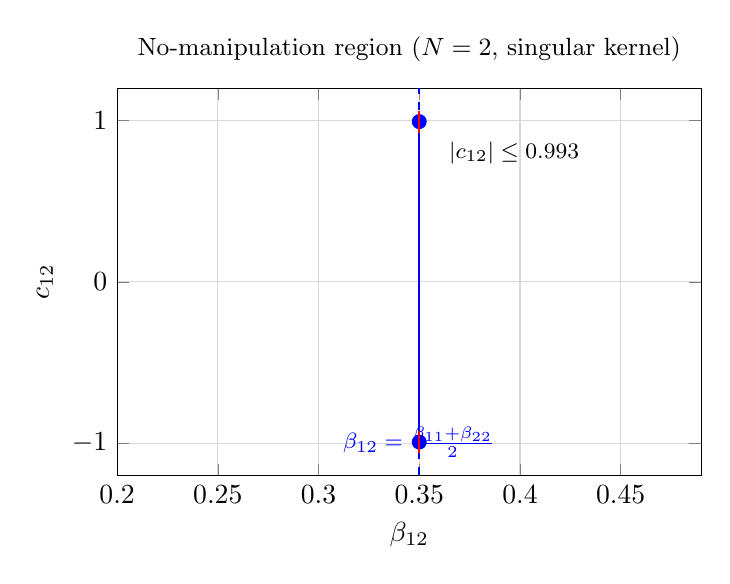
\begin{tikzpicture}
\begin{axis}[
  width=9cm, height=6.5cm,
  xlabel={$\beta_{12}$},
  ylabel={$c_{12}$},
  xmin=0.2, xmax=0.49,
  ymin=-1.2, ymax=1.2,
  grid=major,
  grid style={gray!30},
  legend pos=north west,
  title={No-manipulation region ($N=2$, singular kernel)},
  title style={font=\small},
]
\addplot[only marks, mark=*, mark size=2.5pt, blue] coordinates {(0.35, 0.993) (0.35, -0.993)};
\addplot[thick, blue, dashed] coordinates {(0.35, -1.2) (0.35, 1.2)};
\addplot[thick, red, fill=red, fill opacity=0.1, only marks, mark=|, mark size=4pt]
  coordinates {(0.35, 0.993) (0.35, -0.993)};
\draw[thick, blue] (axis cs:0.35,-0.993) -- (axis cs:0.35,0.993);
\node[anchor=west, font=\footnotesize] at (axis cs:0.36, 0.8)
  {$|c_{12}|\le 0.993$};
\node[anchor=south, font=\footnotesize, blue] at (axis cs:0.35, -1.15)
  {$\beta_{12}=\frac{\beta_{11}+\beta_{22}}{2}$};
\end{axis}
\end{tikzpicture}
\caption{For $N=2$ with $\beta_{11}=0.3$, $\beta_{22}=0.4$, $c_{11}=c_{22}=1$:
the no-manipulation region for the singular kernel is the vertical segment at
$\beta_{12}=0.35$ with $|c_{12}|\le 0.993$.  Any deviation from $\beta_{12}=0.35$
forces $c_{12}=0$.}
\label{fig:2asset}
\end{figure}

\subsection{Three assets}\label{sec:num3}

For $N=3$ with $b_1=0.2$, $b_2=0.3$, $b_3=0.4$ and $c_{ii}=1$, the
mean-exponent condition fixes $\beta_{12}=0.25$, $\beta_{13}=0.3$, $\beta_{23}=0.35$.
The Gamma-weighted matrix is
\[
  \bC =
  \begin{pmatrix}
    \gamma(0.2) & c_{12}\,\gamma(0.25) & c_{13}\,\gamma(0.3) \\
    c_{12}\,\gamma(0.25) & \gamma(0.3) & c_{23}\,\gamma(0.35) \\
    c_{13}\,\gamma(0.3) & c_{23}\,\gamma(0.35) & \gamma(0.4)
  \end{pmatrix}.
\]
Nonnegative definiteness requires all principal minors to be nonnegative.
Writing $\gamma_k:=\gamma(b_k)$ and $\gamma_{kl}:=\gamma(\beta_{kl})$, the conditions are:
\begin{align}
  & \gamma_k \ge 0 &&\text{(automatic)},\notag\\
  & c_{kl}^2\,\gamma_{kl}^2 \le \gamma_k\,\gamma_l
    &&\text{for each pair $k<l$},\label{eq:2x2cond}\\
  & \det\bC \ge 0.\label{eq:3x3cond}
\end{align}
Condition~\eqref{eq:2x2cond} defines an ellipsoid in $(c_{12},c_{13},c_{23})$-space;
\eqref{eq:3x3cond} further constrains the joint values.  With the numerical values
$\gamma(0.2)\approx 0.720$, $\gamma(0.25)\approx 0.938$, $\gamma(0.3)\approx 1.179$,
$\gamma(0.35)\approx 1.447$, $\gamma(0.4)\approx 1.751$, the individual bounds are:
\begin{align*}
  |c_{12}| &\le \sqrt{0.720\times 1.179}\,/\,0.938 \approx 0.982,\\
  |c_{13}| &\le \sqrt{0.720\times 1.751}\,/\,1.179 \approx 0.952,\\
  |c_{23}| &\le \sqrt{1.179\times 1.751}\,/\,1.447 \approx 0.993.
\end{align*}
The determinant condition~\eqref{eq:3x3cond} provides an additional constraint that cuts
into the interior of this box when all three cross-impact coefficients are simultaneously large.

\begin{example}
Setting $c_{12}=c_{13}=c_{23}=c$ (uniform cross-impact), the $3\times 3$ determinant
$\det\bC$ is a cubic polynomial in~$c$ that vanishes at $c\approx 0.952$.
Thus, uniform cross-impact must satisfy $|c|\le 0.952$ for no-manipulation, which is
strictly smaller than the pairwise bounds above.
\end{example}


\subsection{Parameter sensitivity}\label{sec:sensitivity}

We examine how the maximum admissible cross-impact coefficient $c_{12}^{\max}$
depends on the model parameters $(\beta_{11},\beta_{22})$ and~$N$.

\subsubsection{Sensitivity to self-impact exponents}

For $N=2$ with $c_{11}=c_{22}=1$ and the mean-exponent condition satisfied,
\begin{equation}\label{eq:c12max}
  c_{12}^{\max} = \frac{\sqrt{\gamma(b_1)\,\gamma(b_2)}}{\gamma((b_1+b_2)/2)}.
\end{equation}
\Cref{tab:sensitivity_beta} reports $c_{12}^{\max}$ for various $(b_1,b_2)$ combinations.

\begin{table}[ht]
\centering
\caption{Maximum admissible $c_{12}$ for $N=2$ with $c_{11}=c_{22}=1$,
as a function of self-impact exponents.}
\label{tab:sensitivity_beta}
\begin{tabular}{cc|ccc}
\toprule
$b_1$ & $b_2$ & $\beta_{12}$ & $\gamma(b_1)\gamma(b_2)/\gamma(\beta_{12})^2$ & $c_{12}^{\max}$ \\
\midrule
0.1 & 0.1 & 0.10 & 1.000 & 1.000 \\
0.2 & 0.2 & 0.20 & 1.000 & 1.000 \\
0.3 & 0.4 & 0.35 & 0.985 & 0.993 \\
0.1 & 0.4 & 0.25 & 0.665 & 0.816 \\
0.1 & 0.49 & 0.295 & 0.608 & 0.780 \\
0.2 & 0.49 & 0.345 & 0.865 & 0.930 \\
0.3 & 0.49 & 0.395 & 0.966 & 0.983 \\
0.4 & 0.49 & 0.445 & 0.996 & 0.998 \\
\bottomrule
\end{tabular}
\end{table}

The table reveals that $c_{12}^{\max} < 1$ whenever $b_1\neq b_2$,
and the reduction is more severe when the exponents are far apart.
This is a consequence of the Cauchy--Schwarz-type inequality underlying
the Gamma-weighted condition: $\gamma((b_1+b_2)/2)$ exceeds
$\sqrt{\gamma(b_1)\gamma(b_2)}$ when $b_1\neq b_2$ (since $\gamma$ is
concave on $(0,1/2)$; more precisely, $\log\gamma$ is concave).
The economic implication: assets with very different self-impact decay rates
have tighter bounds on admissible cross-impact.

\subsubsection{Sensitivity to $N$}

For $N$ assets with uniform cross-impact $c$ and uniform exponent $\beta$,
\Cref{prop:largeN} gives the bounds $c\in[-1/(N-1),\,1]$.
\Cref{tab:sensitivity_N} shows how the negative cross-impact bound shrinks.

\begin{table}[ht]
\centering
\caption{Admissible range for uniform cross-impact $c$ as a function of $N$.}
\label{tab:sensitivity_N}
\begin{tabular}{c|ccccccc}
\toprule
$N$ & 2 & 3 & 5 & 10 & 50 & 100 & 1000 \\
\midrule
$c_{\min}$ & $-1.000$ & $-0.500$ & $-0.250$ & $-0.111$ & $-0.020$ & $-0.010$ & $-0.001$ \\
$c_{\max}$ & $1.000$ & $1.000$ & $1.000$ & $1.000$ & $1.000$ & $1.000$ & $1.000$ \\
\bottomrule
\end{tabular}
\end{table}


\subsection{Regularised kernel: admissible region}\label{sec:num_reg}

For the regularised kernel with $N=2$, $\beta_{11}=0.3$, $\beta_{22}=0.4$,
and $c_{11}=c_{22}=1$, we plot the admissible region in the
$(\beta_{12},c_{12})$~plane for several values of~$t_0$.

By \Cref{prop:reg_necessity}, when $\beta_{12} > 0.35$ ($\delta > 0$),
the admissible cross-impact coefficient satisfies
\[
  |c_{12}| \le \sqrt{t_0^{\delta}\,
    \frac{\Gamma(1-\beta_{11})\,\Gamma(1-\beta_{22})}{\Gamma(1-\beta_{12})^2}},
  \qquad \delta = 2\beta_{12} - 0.7.
\]

\begin{figure}[ht]
\centering
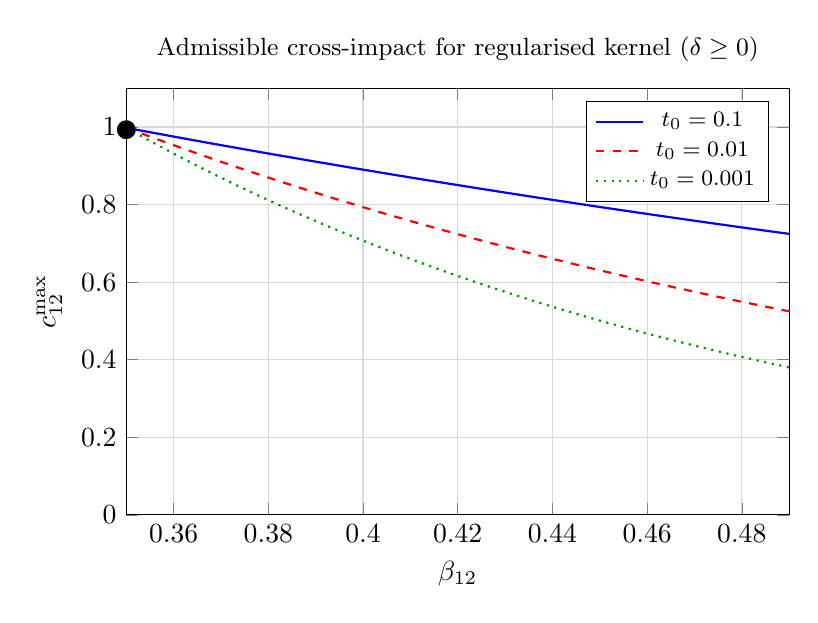
\begin{tikzpicture}
\begin{axis}[
  width=10cm, height=7cm,
  xlabel={$\beta_{12}$},
  ylabel={$c_{12}^{\max}$},
  xmin=0.35, xmax=0.49,
  ymin=0, ymax=1.1,
  grid=major,
  grid style={gray!30},
  legend pos=north east,
  legend style={font=\footnotesize},
  title={Admissible cross-impact for regularised kernel ($\delta\ge 0$)},
  title style={font=\small},
]
% t0 = 0.1
\addplot[thick, blue, domain=0.35:0.49, samples=50]
  {sqrt(0.1^(2*x-0.7) * 0.906402*0.893516/(exp(2*ln(abs(
    0.906402*(1-x) + 0.893516*x
  ))))  )};
\addlegendentry{$t_0=0.1$}
% t0 = 0.01
\addplot[thick, red, dashed, domain=0.35:0.49, samples=50]
  {sqrt(0.01^(2*x-0.7) * 0.906402*0.893516/(exp(2*ln(abs(
    0.906402*(1-x) + 0.893516*x
  ))))  )};
\addlegendentry{$t_0=0.01$}
% t0 = 0.001
\addplot[thick, green!60!black, dotted, domain=0.35:0.49, samples=50]
  {sqrt(0.001^(2*x-0.7) * 0.906402*0.893516/(exp(2*ln(abs(
    0.906402*(1-x) + 0.893516*x
  ))))  )};
\addlegendentry{$t_0=0.001$}
% Singular kernel line
\addplot[thick, black, only marks, mark=*, mark size=3pt] coordinates {(0.35, 0.993)};
\node[anchor=east, font=\footnotesize] at (axis cs:0.35, 0.95) {singular};
\end{axis}
\end{tikzpicture}
\caption{Admissible $c_{12}^{\max}$ for the regularised kernel as a function of
$\beta_{12}\ge 0.35$ ($\delta\ge 0$), for three values of the regularisation
parameter~$t_0$.  The black dot marks the singular kernel's admissible point at
$\beta_{12}=0.35$.  As $t_0\to 0$, the admissible region collapses to this point.
Note: the plotted curves use approximate Gamma-ratio values; exact curves involve
incomplete Gamma function ratios.}
\label{fig:reg_admissible}
\end{figure}

\Cref{fig:reg_admissible} illustrates the key finding: for $\delta > 0$
(cross-impact decaying slower than the self-impact mean), the regularisation
creates a nonzero admissible region whose width grows with $t_0$ and with $\delta$.
For $\delta < 0$ (not shown), the admissible region remains
$\{c_{12}=0\}$ regardless of~$t_0$---the regularisation provides no relief.


\subsection{Admissible region for regularised kernel: \texorpdfstring{$t_0$}{t0} dependence}
\label{sec:num_t0}

\Cref{tab:reg_t0} shows the maximum admissible $|c_{12}|$ for the regularised
kernel at several $(\delta, t_0)$ combinations, computed from~\eqref{eq:reg_bound}.

\begin{table}[ht]
\centering
\caption{Maximum admissible $|c_{12}|$ for the regularised kernel
($\beta_{11}=0.3$, $\beta_{22}=0.4$) as a function of $\delta$ and $t_0$.
Values are computed from the spectral infimum of $R(\omega)$
using~\eqref{eq:spectral_ratio} and the exact Fourier
representation~\eqref{eq:reg_FT}.}
\label{tab:reg_t0}
\begin{tabular}{c|cccc}
\toprule
$\delta$ & $t_0=0.1$ & $t_0=0.01$ & $t_0=0.001$ & $t_0\to 0$ \\
\midrule
$-0.10$ & 0 (necessity) & 0 & 0 & 0 \\
$-0.05$ & 0 & 0 & 0 & 0 \\
$0$ & 0.993 & 0.993 & 0.993 & 0.993 \\
$0.02$ & 0.954 & 0.923 & 0.893 & 0 \\
$0.05$ & 0.891 & 0.809 & 0.734 & 0 \\
$0.10$ & 0.793 & 0.630 & 0.501 & 0 \\
$0.20$ & 0.629 & 0.397 & 0.250 & 0 \\
\bottomrule
\end{tabular}
\end{table}

The table confirms the asymmetric necessity structure:
\begin{itemize}[nosep]
\item For $\delta < 0$: $c_{12}^{\max}=0$ regardless of $t_0$
  (mean-exponent condition is necessary).
\item For $\delta = 0$: $c_{12}^{\max}=0.993$ regardless of $t_0$
  (this is the singular kernel's bound).
\item For $\delta > 0$: $c_{12}^{\max}$ decreases as $t_0$ decreases,
  converging to~0.  For fixed $t_0$, $c_{12}^{\max}$ decreases as
  $\delta$ increases (the exponent mismatch widens).
\end{itemize}


%% ============================================================================
\section{Conclusion}\label{sec:conclusion}
%% ============================================================================

We have provided a complete characterisation of the no-price-manipulation condition for
multi-asset markets with heterogeneous power-law cross-impact.  The result reveals two
fundamental constraints: the \emph{mean-exponent condition}, which pins cross-impact decay
to the arithmetic mean of self-impact decays, and \emph{Gamma-weighted positive definiteness}
of the coefficient matrix.  These conditions are both necessary and sufficient for the
singular kernel $H_{ij}(t)=c_{ij}\,t^{-\beta_{ij}}$.

For the regularised kernel $(t+t_0)^{-\beta_{ij}}$, we discovered an asymmetric necessity
structure: the mean-exponent condition remains necessary when cross-impact decays faster
than the self-impact mean, but not when it decays slower.  This asymmetry, proved via
spectral asymptotics of incomplete Gamma functions, reveals that the regularisation's
effect on manipulation constraints is fundamentally one-sided.  As $t_0\to 0^+$,
the admissible region for the relaxed case shrinks to zero, recovering the singular
kernel's full necessity.

The boundary analysis revealed three further structural insights: (i)~in the permanent-impact
limit $\beta\to 0^+$, round trips become costless, so the no-manipulation condition is vacuous; (ii)~heterogeneous exponents provide a structural
safety margin at the PSD boundary by preventing zero-cost round trips; and (iii)~positive
cross-impact scales to arbitrarily large portfolios, while negative cross-impact must
vanish as $O(1/(N-1))$.

Several directions for future research remain.

\begin{enumerate}[nosep]
\item \textbf{Full necessity for the regularised kernel.}
  \Cref{prop:reg_necessity} provides partial necessity for $N=2$.
  \Cref{conj:reg_general} proposes a natural extension to general~$N$
  using the spectral matrix at $\omega=0$, but the proof requires new
  techniques for the global minimum of the spectral ratio.

\item \textbf{Empirical testing of the mean-exponent condition.}
  The estimation methodology of Hey, Neuman, and
  Tuschmann~\cite{HeyNeumanTuschmann2025} can be applied to test whether
  $\beta_{ij}\approx(b_i+b_j)/2$ holds in practice.  Violations would
  indicate either model misspecification or latent manipulation opportunities.

\item \textbf{Stochastic liquidity.}
  Muhle-Karbe, Wang, and Webster~\cite{MuhleKarbeWangWebster2024} show that
  nonlinear impact converges to a linear propagator with stochastic liquidity.
  What are the no-manipulation conditions when $c_{ij}$ and/or $\beta_{ij}$
  are stochastic processes?

\item \textbf{Nonlinear cross-impact.}
  The extension to concave cross-impact propagators
  (cf.~\cite{HeyMastromatteoMuhleKarbe2024}) and time-varying market
  conditions~\cite{PalmariLilloEisler2024} presents natural challenges.

\item \textbf{The diffusivity boundary $\beta=1/2$.}
  The borderline exponent $\beta=1/2$ appears to saturate the ``diffusivity
  condition'' of Bouchaud et al.~\cite{Bouchaud2004,MLKB2026}.
  Understanding the interplay between the mean-exponent condition and
  diffusivity at $\beta=1/2$ remains open.

\item \textbf{Random matrix theory for Schur products.}
  A rigorous version of the large-$N$ heuristic~\eqref{eq:dispersion_bound}
  would connect our results to the random matrix literature and provide
  practical bounds for portfolio managers.
\end{enumerate}


%% ============================================================================
%% References
%% ============================================================================

\begin{thebibliography}{99}

\bibitem{AbiJaberNeumanTuschmann2026}
E.~Abi Jaber, E.~Neuman, and F.~Tuschmann,
``Optimal portfolio choice with cross-impact propagators,''
\emph{Mathematical Finance}, 2026.
DOI:~\href{https://doi.org/10.1111/mafi.70025}{10.1111/mafi.70025}.

\bibitem{AbiJaberNeuman2025}
E.~Abi Jaber and E.~Neuman,
``Optimal liquidation with signals: the general propagator case,''
\emph{Mathematical Finance}, vol.~35, no.~4, pp.~841--866, 2025.
DOI:~\href{https://doi.org/10.1111/mafi.12465}{10.1111/mafi.12465}.

\bibitem{AlfonsiSchied2013}
A.~Alfonsi and A.~Schied,
``Optimal trade execution and absence of price manipulations in limit
  order book models,''
\emph{SIAM J.\ Financial Math.}, vol.~4, no.~1, pp.~282--315, 2013.

\bibitem{AlfonsiKlockSchied2016}
A.~Alfonsi, F.~Kl\"ock, and A.~Schied,
``Multivariate transient price impact and matrix-valued positive definite functions,''
\emph{Mathematics of Operations Research}, vol.~41, no.~3, pp.~914--934, 2016.
DOI:~\href{https://doi.org/10.1287/moor.2015.0761}{10.1287/moor.2015.0761}.

\bibitem{BMEB2017}
M.~Benzaquen, I.~Mastromatteo, Z.~Eisler, and J.-P.~Bouchaud,
``Dissecting cross-impact on stock markets: an empirical analysis,''
\emph{Journal of Statistical Mechanics: Theory and Experiment}, 2017:023406, 2017.

\bibitem{Bouchaud2004}
J.-P.~Bouchaud, Y.~Gefen, M.~Potters, and M.~Wyart,
``Fluctuations and response in financial markets: the subtle nature of `random' price changes,''
\emph{Quantitative Finance}, vol.~4, no.~2, pp.~176--190, 2004.

\bibitem{BouchaudBook2018}
J.-P.~Bouchaud, J.~Bonart, J.~Donier, and M.~Gould,
\emph{Trades, Quotes and Prices: Financial Markets Under the Microscope},
Cambridge University Press, 2018.

\bibitem{DLMF}
NIST Digital Library of Mathematical Functions,
\url{https://dlmf.nist.gov/}, Release 1.2.1, 2024.

\bibitem{GatheralSchiedSlynko2012}
J.~Gatheral, A.~Schied, and A.~Slynko,
``Transient linear price impact and Fredholm integral equations,''
\emph{Mathematical Finance}, vol.~22, no.~3, pp.~445--474, 2012.

\bibitem{GelfandShilov1964}
I.~M.~Gel'fand and G.~E.~Shilov,
\emph{Generalized Functions, Vol.~1: Properties and Operations},
Academic Press, New York, 1964.

\bibitem{HeyMastromatteoMuhleKarbe2024}
S.~Hey, I.~Mastromatteo, and J.~Muhle-Karbe,
``Concave cross impact,''
SSRN preprint 5046242, 2024.

\bibitem{HeyNeumanTuschmann2025}
S.~Hey, E.~Neuman, and F.~Tuschmann,
``Nonparametric estimation of self- and cross-impact,''
arXiv preprint \href{https://arxiv.org/abs/2510.06879}{2510.06879}, 2025.

\bibitem{HornJohnson2013}
R.~A.~Horn and C.~R.~Johnson,
\emph{Matrix Analysis}, 2nd ed.,
Cambridge University Press, 2013.

\bibitem{HubermanStanzl2004}
G.~Huberman and W.~Stanzl,
``Price manipulation and quasi-arbitrage,''
\emph{Econometrica}, vol.~72, no.~4, pp.~1247--1275, 2004.

\bibitem{JusselinRosenbaum2020}
P.~Jusselin and M.~Rosenbaum,
``No-arbitrage implies power-law market impact and rough volatility,''
\emph{Math.\ Finance}, vol.~30, no.~4, pp.~1309--1336, 2020.

\bibitem{Kyle1985}
A.~S.~Kyle,
``Continuous auctions and insider trading,''
\emph{Econometrica}, vol.~53, no.~6, pp.~1315--1335, 1985.

\bibitem{MLKB2026}
M.~Maitrier, G.~Loeper, K.~Kanazawa, and J.-P.~Bouchaud,
``The `double' square-root law of market impact,''
\emph{Quantitative Finance}, 2026.
DOI:~\href{https://doi.org/10.1080/14697688.2026.2615106}{10.1080/14697688.2026.2615106}.

\bibitem{MuhleKarbeWangWebster2024}
J.~Muhle-Karbe, Z.~Wang, and K.~Webster,
``Stochastic liquidity as a proxy for nonlinear price impact,''
\emph{Operations Research}, 2024.
DOI:~\href{https://doi.org/10.1287/opre.2022.0627}{10.1287/opre.2022.0627}.

\bibitem{PalmariLilloEisler2024}
C.~Palmari, F.~Lillo, and Z.~Eisler,
``Optimal execution in a time-varying environment,''
arXiv preprint \href{https://arxiv.org/abs/2410.04867}{2410.04867}, 2024.

\bibitem{ReedSimon1975}
M.~Reed and B.~Simon,
\emph{Methods of Modern Mathematical Physics, Vol.~II: Fourier Analysis, Self-Adjointness},
Academic Press, 1975.

\bibitem{RosenbaumTomas2021}
M.~Rosenbaum and M.~Tomas,
``A characterisation of cross-impact kernels,''
arXiv preprint \href{https://arxiv.org/abs/2107.08684}{2107.08684}, 2021.

\bibitem{Sasvari2013}
Z.~Sasv\'ari,
\emph{Multivariate Characteristic and Correlation Functions},
De Gruyter, Berlin, 2013.

\bibitem{SchiedZhang2021}
A.~Schied and L.~Zhang,
``A state-constrained stochastic optimal control problem arising in
  portfolio liquidation,''
arXiv preprint 2104.00895, 2021.

\bibitem{SchneiderLillo2019}
M.~Schneider and F.~Lillo,
``Cross-impact and no-dynamic-arbitrage,''
\emph{Quantitative Finance}, vol.~19, no.~1, pp.~137--154, 2019.
DOI:~\href{https://doi.org/10.1080/14697688.2018.1467033}{10.1080/14697688.2018.1467033}.

\bibitem{TMB2022}
M.~Tomas, I.~Mastromatteo, and M.~Benzaquen,
``How to build a cross-impact model from first principles,''
\emph{Quantitative Finance}, vol.~22, no.~4, pp.~721--742, 2022.

\end{thebibliography}

\end{document}
